\documentclass[11pt,a4paper]{article}

% ---------------------------------------------------------------------------
% Basic packages
% ---------------------------------------------------------------------------
\usepackage[margin=1in]{geometry}
\usepackage{amsmath, amssymb, amsfonts}
\usepackage{bm}
\usepackage{graphicx}
\usepackage{booktabs}
\usepackage{hyperref}
\usepackage[numbers,sort&compress]{natbib}
\usepackage{caption}
\usepackage{subcaption}
\usepackage{mathtools}
\usepackage{xcolor}
\usepackage{lmodern}
\usepackage{tikz}
\graphicspath{{figures/}}

% ---------------------------------------------------------------------------
% Hyperref setup
% ---------------------------------------------------------------------------
\hypersetup{
    colorlinks=true,
    linkcolor=blue,
    citecolor=blue,
    urlcolor=blue,
    pdftitle={An Information-Theoretic Framework for Vertebral Morphogenesis},
    pdfauthor={Dr. Sayuj Krishnan S},
}

% ---------------------------------------------------------------------------
% Macros for recurring notation
% ---------------------------------------------------------------------------
% Fields and functions
\newcommand{\Ifield}{I(s)}
\newcommand{\Ifieldt}{I(s,t)}
\newcommand{\gEff}{g_{\mathrm{eff}}}
\newcommand{\Dgeo}{D_{\mathrm{geo}}}
\newcommand{\Dgeohat}{\widehat{D}_{\mathrm{geo}}}
\newcommand{\kappaPassive}{\kappa_{0}}
\newcommand{\kappaInfo}{\kappa_{I}}
\newcommand{\chiK}{\chi_{\kappa}}
\newcommand{\chiE}{\chi_{E}}
\newcommand{\chiC}{\chi_{C}}
\newcommand{\chiM}{\chi_{\kappa}}

% Metric and line element
\newcommand{\dlEff}{d\ell_{\mathrm{eff}}}
\newcommand{\metricEff}{\dlEff^{2} = \gEff(s)\,ds^{2}}

% Scoliosis metrics
\newcommand{\Slat}{S_{\mathrm{lat}}}
\newcommand{\Cobb}{\theta_{\mathrm{Cobb}}}

% Nonlocal sliding (counterbend mechanics)
\newcommand{\muSliding}{\mu}
\newcommand{\gammaCompliance}{\gamma}

% Information Theory notation
\newcommand{\ShannonH}{\mathcal{H}}
\newcommand{\KLDivergence}{D_{\mathrm{KL}}}
\newcommand{\FisherInfo}{\mathcal{F}}
\newcommand{\InstabilityR}{R(t)}

% Misc
\newcommand{\Reals}{\mathbb{R}}
\newcommand{\dd}{\mathrm{d}}

% ---------------------------------------------------------------------------
% Mathematical Box environment Fallback
% ---------------------------------------------------------------------------
\newenvironment{mathbox}[1][]
 {\par\vspace{\baselineskip}\noindent\textbf{#1}\par\noindent\rule{\textwidth}{0.4pt}\par\noindent}
 {\par\noindent\rule{\textwidth}{0.4pt}\vspace{\baselineskip}\par}

% ---------------------------------------------------------------------------
% Title / Authors
% ---------------------------------------------------------------------------
\title{Biological Counter-Curvature: An Information--Cosserat Framework for Vertebral Geometry and Adolescent Scoliosis}

\author{Dr.~Sayuj Krishnan S, MBBS, DNB (Neurosurgery)\\
Consultant Neurosurgeon and Spine Surgeon, Yashoda Hospitals, Malakpet, Hyderabad, India\\
\texttt{dr.sayujkrishnan@gmail.com}
}

\date{\today}

% ---------------------------------------------------------------------------
% Document
% ---------------------------------------------------------------------------
\begin{document}
\maketitle


% START INPUT: sections/abstract.tex
\begin{abstract}
Adolescent Idiopathic Scoliosis (AIS) is a complex 3D skeletal failure, yet the physical principles governing its onset remain elusive. We propose a unifying framework, "Biological Countercurvature," which explains how the human spine actively maintains its sagittal profile against gravity through Information--Elasticity Coupling (IEC). Using 3D Cosserat rod mechanics and AlphaFold-derived protein structural metrics, we demonstrate that the spinal S-curve is an active, energy-demanding morphoelastic target encoded by developmental information fields. We identify a fundamental "Gravity Paradox" wherein the mechanical cost of maintaining this counter-curvature ($L^4$) outpaces metabolic diffusion supply ($L^2$) during rapid growth. This scaling mismatch precipitates a "Thermodynamic Buckling" window, where the spine collapses into a scoliosis-like mode to minimize entropy. Our results suggest that AIS represents an "Information Loss" catastrophe caused by the metabolic insolvency of the developmental information channel during puberty.
\end{abstract}

% END INPUT: sections/abstract.tex

% \input{sections/significance}

% START INPUT: sections/introduction.tex
\section{Introduction}

\subsection{Background: Gravity as a Morphogenetic Cue}
Life on Earth has evolved within the unyielding context of a constant gravitational field ($g \approx 9.81 \, m/s^2$). The human sagittal profile---characterized by an alternating sequence of lordosis and kyphosis---actively maintains regional alignment and global balance against gravity. This complex geometry is energetically demanding and non-intuitive under purely passive mechanical models. While conservative treatments (e.g., rigid bracing) heavily rely on passive external correction~\cite{negus_bracing}, they often fail to capture the active morphoelastic dynamics governing the spine.

Traditional biomechanical paradigms, such as the Hueter-Volkmann principle and asymmetric mechanical loading models~\cite{stokes2006hueter}, describe the progression of spinal deformities. However, they struggle to fully explain the rapid, 3D etiologic onset of Adolescent Idiopathic Scoliosis (AIS). Bridging the gap between macroscopic global alignment and tissue-level mechanotransduction remains a critical challenge.

\subsection{Bridge: Information-Elasticity Coupling \& The Gravity Paradox}
To address this ``Translation Problem'' between 1D genetic codes (e.g., HOX clusters~\cite{wellik2007hox}) and 3D geometric alignment, we developed an \textbf{Information-Elasticity Coupling (IEC)} framework. Rather than a purely passive structure, the spine operates under continuous developmental signals that drive localized tissue-remodeling. These signals generate morphoelastic target geometries---a ``Biological Countercurvature''---governing active tissue-level mechanobiological reference states.

However, this active structural maintenance is highly vulnerable. We define the \textbf{Gravity Paradox}: a fundamental scaling dilemma related to the adolescent growth spurt. As the spine undergoes rapid axial elongation, the mechanical moment required to counteract gravity scales as length to the fourth power ($L^4$). Concurrently, the diffusive nutrient supply traversing the avascular intervertebral disc endplate scales strictly as surface area ($L^2$)~\cite{urban2004nutrition}. This $L^4$ vs $L^2$ divergence forces a critical ``Energy Deficit Window,'' initiating an inevitable sequence of structural compromises.

In this deficit regime, the system must prioritize survival over geometry. High-fidelity mechanosensors like Piezo2~\cite{wang2020piezo2} and the LINC complex (Lamin A/C)~\cite{cheng2019lamin}, which are structurally expensive to maintain due to their high anisotropy, are downregulated or decoupled. This loss of sensory precision leads to ``Spinal Jetlag''---a desynchronization between the internal biological clock and volumetric growth. The result is a buckling instability: the spine abandons the metabolically expensive S-shape and relaxes into a lower-energy, gravity-dominated C-shape or the helical torsion of scoliosis.

\subsection{Testable Predictions}
This framework yields specific, falsifiable predictions regarding the etiology of spinal deformity and adaptation to microgravity, grounded in the thermodynamic cost of maintaining the biological counter-curvature standing wave:

\begin{enumerate}
    \item \textbf{The Frequency-Hypoxia Coupling and Convective Shutdown}: We predict that the intervertebral disc (IVD) operates as a convective-diffusive pump where solute transport depends on the frequency ($f_{\mathrm{load}}$) and amplitude of postural changes. Below a critical threshold ($\InstabilityR > 1$), we predict a ``Convective Shutdown'' where reduced fluid exchange triggers a hypoxic switch (HIF-1$\alpha$ stabilization). This predicts that paraspinal muscle biopsies in rapid AIS progressors will show elevated p21 (growth arrest) and MMP1/3 activity localized to the apex of the curve, even prior to structural collapse~\cite{chen2025mmp, sato2025convective}.

    \item \textbf{Small-Molecule Rescue of the Energy Deficit}: If scoliosis is driven by the $L^4/L^2$ metabolic deficit, alignment should be rescuable by metabolic buffering rather than mechanical force. We predict that chronotherapy (e.g., the clock enhancer Nobiletin) or pH-buffering agents will restore SIRT1/PGC-1$\alpha$ signaling and prevent the degradation of high-anisotropy sensors like Piezo2. In bovine IVD cultures under static load, these agents should prevent the loss of BMAL1-driven matrix turnover~\cite{he2016nobiletin, yang2017circadian}.

    \item \textbf{The Spinal Phase Shift ($\Delta \phi$)}: We predict a measurable lag between the central SCN clock and the peripheral spinal clock in AIS patients. This ``Spinal Jetlag'' ($\Delta \phi$) arises because the proprioceptive update rate for high-anisotropy sensors (Lamin A/C, Piezo2) cannot keep pace with the $L^3$ volumetric growth spurt. We predict that $\Delta \phi$ will be a superior predictor of curve progression than the Risser sign, with a phase difference exceeding 4 hours marking the point of irreversible scoliotic buckling~\cite{dudek2017clock}.
\end{enumerate}

In the following sections, we formalize this theory using Cosserat rod mechanics, demonstrating how minimizing the Free Energy of the spine ($U_{CC}$) naturally emerges the S-shaped geometry and how metabolic deficits lead to scoliotic buckling.

% END INPUT: sections/introduction.tex

% START INPUT: sections/theory.tex
\section{Theory}

We propose that the robust S-shaped geometry of the spine arises not from passive mechanical equilibrium under gravity, but from an active \emph{counter-curvature} mechanism driven by developmental information. We formalize this using an Information--Elasticity Coupling (IEC) framework, where a scalar information field $I(s)$ modifies the effective geometry and energetics of a Cosserat rod.

\subsection{The Counter-Curvature Hypothesis}

The central problem of vertebrate morphogenesis is the translation of a one-dimensional genetic code into a robust three-dimensional geometry that can withstand environmental loads. In the case of the human spine, this challenge is acute: the column must support the head and trunk against the relentless downward pull of gravity ($g \approx 9.81$ m/s$^2$) while maintaining flexibility for locomotion. Classical structural mechanics predicts that a flexible column clamped at the base and subjected to its own weight will buckle or sag into a monotonic C-shape~\cite{goriely2017mathematics}. Yet, the healthy human spine exhibits a complex, alternating S-shape (lordosis and kyphosis).

This anomaly suggests that the S-shape is not a passive equilibrium but an active \emph{Counter-Curvature}---a geometric standing wave maintained by the continuous expenditure of metabolic energy against the gravitational field. This hypothesis bridges two foundational concepts in biology: the \emph{Morphogenetic Field} of developmental biology~\cite{wolpert1969positional, saunders1948proximodistal} and the \emph{Mechanostat} of tissue physiology~\cite{frost1987mechanostat}.

\paragraph{The Information Field as a Target Metric.}
Developmental patterning establishes a "Positional Information" field along the anterior-posterior axis, encoded by the nested expression of HOX genes~\cite{wellik2007hox}. We posit that this information field $I(s)$ does not merely specify cell identity but encodes a \emph{target metric}---a preferred intrinsic curvature $\kappa_{rest}(s)$ that the tissue strives to achieve. This is analogous to the "growth field" concepts in plant morphogenesis~\cite{coen2004war} but applied to a load-bearing animal structure. The spine is thus a "smart beam" that continuously computes the error between its actual geometry (sensed via proprioception) and its genetic target.

\paragraph{Active Maintenance and the Hydrostatic Skeleton.}
Achieving this target shape against gravity requires work. The spine functions partly as a \emph{hydrostatic skeleton}~\cite{kier1985hydrostatic}, where the nucleus pulposus of the intervertebral disc acts as a pressurized hydraulic element. The maintenance of this pressure---and thus the maintenance of the S-shape---depends on the balance between osmotic swelling pressure (driven by proteoglycan synthesis) and the mechanical stress of gravity. This active maintenance constitutes a biological implementation of \emph{optimal feedback control}~\cite{todorov2002optimal}, where the system minimizes a cost function comprising both "geometric error" (deviation from the HOX-specified shape) and "metabolic effort" (ATP consumption).

\paragraph{Predictions.}
This unifying hypothesis generates three testable predictions that distinguish it from purely mechanical buckling models:
\begin{enumerate}
    \item \textbf{Frequency-Hypoxia Coupling}: We predict that the maintenance of the S-shape requires dynamic loading frequencies $>0.5$ Hz to drive convective transport. Reducing frequency (e.g., microgravity) will stabilize HIF-1$\alpha$ in the nucleus pulposus before any structural deformity appears~\cite{ugur2024hypoxia}.
    \item \textbf{The "Small-Molecule Rescue"}: If scoliotic buckling is a metabolic failure (Energy Deficit), then enhancing the amplitude of the circadian clock (e.g., via Nobiletin) or buffering local pH should restore spinal alignment even without mechanical correction.
    \item \textbf{The Spinal Phase Shift}: The severity of spinal curvature should correlate with the phase lag between the central (SCN) and peripheral (IVD) circadian clocks, providing a quantifiable biomarker for "Counter-Curvature" failure.
\end{enumerate}

\subsection{Rod Geometry and Kinematics} \label{sec:rod_geometry}
(See Supplementary Material for full Cosserat formulation).

\subsection{Developmental Information Fields from Morphogenetic Patterning}

We introduce a scalar information field $I(s, t) \in [0, 1]$ representing the coarse-grained expression level of anterior-posterior patterning morphogens (e.g., HOX genes). This field serves as a coarse-grained representation of the complex gene regulatory networks governing axial patterning. Following the bimodal Gaussian parameterization (Methods Eq.~\ref{eq:info_field_spinal}), we model $I(s)$ with peaks at the cervical ($A_c=0.5, s_c=0.80$) and lumbar ($A_l=0.7, s_l=0.25$) enlargements, corresponding to regions of high vertebral identity specification. The spatial gradient $\nabla I$ acts as a "curvature generator" via the geometric coupling $\chi_\kappa$:
\begin{equation}
\boldsymbol{\kappa}_{\mathrm{rest}}(s) = \boldsymbol{\kappa}_{\mathrm{gen}} + \chi_\kappa \nabla I(s).
\label{eq:kappa_rest}
\end{equation}
We quantify the information content of this patterning field using the local Shannon entropy $\ShannonH[I]$, which bounds the precision of the target metric specification:
\begin{equation}
\ShannonH[I] = -\int I(s) \log I(s) \, ds.
\label{eq:shannon_entropy}
\end{equation}
Simultaneously, the field exerts a stiffness via the morphomechanical coupling $\chi_M$, generating the active biological moment $\mathbf{M}_{bio}$ to oppose gravity:
\begin{equation}
\mathbf{M}_{bio} = \chi_M (\mathbf{\Lambda} \cdot \nabla I).
\label{eq:active_moment}
\end{equation}
Stability is quantified by the Bio-Gravitational Number $\mathcal{B}_g$:
\begin{equation}
\mathcal{B}_g = \frac{\chi_M \langle |\nabla I| \rangle}{\rho A g L^2}.
\label{eq:bg_number}
\end{equation}
When $\mathcal{B}_g > 1$, the organism dominates gravity. This framework is physically grounded in the structural specificity of HOX proteins. For example, AlphaFold analysis of HOXC8 (UniProt P31273) and HOXB13 (UniProt Q92826) demonstrates that these proteins possess rigid DNA-binding domains capable of enforcing the sharp identity boundaries necessary for this parameterization.

\subsection{The Information--Cosserat Manifold Framework}
The Human spine is modeled as a one-dimensional Cosserat rod embedded in three-dimensional Euclidean space. In the IEC framework, we treat the rod's reference configuration as a manifold whose intrinsic geometry is defined by a developmental information field $I(s)$. This field specifies the local target curvature $\kappa_{\mathrm{rest}}(s)$, effectively 'shaping' the biological reference state against which elastic deformations are measured. We analyzed the structural specificity of developmental transcription factors; for instance, AlphaFold 3 analysis of HOXC8 (UniProt P31273) and HOXB13 (UniProt Q92826) reveals highly conserved amino acid domains (avg. pLDDT $\sim 64.1$) whose structural rigidity provides the necessary binding affinity landscapes to generate the segmented information profiles used in our model.

\subsection{Biological Metric and the Effective Energy Functional}

The central hypothesis of the IEC framework is that developmental information modifies the \emph{effective} metric experienced by the rod's reference manifold. We define a \emph{biological metric} $d\ell_{\mathrm{eff}}^2$ that encodes target geometry via a local dilation factor $g_{\mathrm{eff}}(s)$:

\begin{equation}
d\ell_{\mathrm{eff}}^2 = g_{\mathrm{eff}}(s)\,ds^2 = \exp\left[2\left(\beta_1 \tilde{I}(s) + \beta_2 \frac{\partial \tilde{I}}{\partial s}\right)\right] ds^2,
\label{eq:biological_metric}
\end{equation}
where $\tilde{I}$ is the normalized information field and $\beta_{1,2}$ are dimensionless coupling constants.

The mechanics of the biological rod are governed by the minimization of a total potential energy $\mathcal{E}_{\mathrm{total}}$ that couples bending, torsion, and extension to the information field and gravity. For a Cosserat rod with centerline $\mathbf{r}(s)$, the full energy functional is:

\begin{equation}
\mathcal{E}_{\mathrm{total}} = \int_0^L \left[ \frac{1}{2} B_{\mathrm{eff}}(\kappa - \kappa_{\mathrm{rest}})^2 + \frac{1}{2} C_{\mathrm{eff}} \tau^2 + \frac{1}{2} K_{\mathrm{eff}} \varepsilon^2 + \rho A \mathbf{r} \cdot \mathbf{g} \right] ds,
\label{eq:iec_energy}
\end{equation}
where:
\begin{itemize}
    \item $B_{\mathrm{eff}}(s) = E_0 I_{\mathrm{area}} (1 + \chi_E I(s))$ is the information-modulated bending stiffness.
    \item $C_{\mathrm{eff}}(s) = G_0 J (1 + \chi_C I(s))$ is the torsional stiffness ($G_0$: shear modulus).
    \item $K_{\mathrm{eff}}(s) = E_0 A (1 + \chi_A I(s))$ is the extensional stiffness.
    \item $\kappa_{\mathrm{rest}}(s) = \kappa_0 + \chi_\kappa \partial_s I$ is the information-driven target curvature.
    \item $\tau$ and $\varepsilon$ are the local torsion and strain, respectively.
\end{itemize}
The weighting $w(I) = (1 + \chi_E I(s))$ penalizes deviations from the information-prescribed counter-curvature more heavily in high-identity regions (e.g., cervical/lumbar junctions). Note that we use $\chi_A$ for area stiffness modulation to distinguish it from the morphomechanical coupling $\chi_M$ defined earlier.

\subsection{Mechanical Equilibrium}
(See Supplementary Material for balance equations and boundary conditions).

\subsection{Mode selection and spinal geometry}

The transition from a sagging C-shape to a counter-curved S-shape can be analyzed as a spectral shift in the rod's eigenmodes. In the linearized limit, small transverse deflections $y(s)$ satisfy:

\begin{equation}
\mathcal{L}_{\mathrm{IEC}}[y(s)] = \frac{d^2}{ds^2} \left( B_{\mathrm{eff}}(s) \frac{d^2 y}{ds^2} \right) - \frac{d}{ds} \left( N(s) \frac{dy}{ds} \right) = \lambda_n y_n(s),
\label{eq:mode_selection}
\end{equation}
where $N(s) = \int_s^L \rho A g \, ds'$ is the axial tension due to gravity. The information field modifies the stiffness landscape $B_{\mathrm{eff}}(s)$. For a uniform beam ($\chi_E = 0$), the lowest eigenvalue $\lambda_0$ corresponds to a monotonic C-shaped mode. As $\chi_\kappa$ and $\chi_E$ increase, the effective stiffness at the peaks of $I(s)$ (cervical and lumbar regions) increases, making the C-mode energetically unfavorable. At a critical coupling strength $\chi_{\mathrm{crit}}$, a \emph{mode crossing} occurs where the S-shaped mode (characterized by a second zero-crossing in curvature) becomes the ground state ($\lambda_0$).

To quantify the degree of biological countercurvature—the extent to which information reshapes equilibrium geometry—we define the Kullback--Leibler (KL) divergence, $\KLDivergence(P_{\mathrm{IEC}} \| P_{\mathrm{passive}})$, between the probability distribution of the IEC-coupled geometry and that of the passive gravitational state:

\begin{equation}
\KLDivergence = \int_0^L \left[ \frac{1}{2} \left( \kappa_{\mathrm{IEC}}(s) - \kappa_{\mathrm{passive}}(s) \right)^2 \FisherInfo(s) \right] w(s)\, ds,
\label{eq:kl_divergence}
\end{equation}
where $\FisherInfo(s)$ is the local Fisher Information and $w(s) = g_{\mathrm{eff}}(s)$ is a weighting function reflecting the biological metric. For regime classification, we normalize by the maximum divergence observed across the parameter space:

\begin{equation}
\Dgeohat = \frac{\KLDivergence}{\KLDivergence^{\mathrm{max}}(\chi_\kappa, g)},
\label{eq:dgeo_normalized}
\end{equation}
where $\KLDivergence^{\mathrm{max}}$ is computed over the explored $(\chi_\kappa, g)$ domain. Physically, $\Dgeohat \approx 0$ indicates the system follows gravitational geodesics (passive regime), while $\Dgeohat \sim 1$ indicates strong information-driven geometric distortion. We classify regimes as: \emph{gravity-dominated} ($\Dgeohat < 0.1$), \emph{cooperative} ($0.1 \leq \Dgeohat \leq 0.3$), and \emph{information-dominated} ($\Dgeohat > 0.3$), with thresholds chosen to separate qualitatively distinct curvature morphologies observed in simulations.

The energy functional $\mathcal{E}_{\mathrm{total}}$ (Eq.~\ref{eq:iec_energy}) describes the potential energy landscape of the spine at equilibrium. However, the biological spine is not a conservative system: it is a \emph{dissipative structure}~\cite{prigogine1977self} that requires continuous metabolic expenditure to maintain its S-shaped counter-curvature against gravitational loading and entropic degradation. According to Landauer's principle, the erasure or maintenance of information $\ShannonH$ carries a minimum metabolic cost of $k_B T \ln 2$ per bit. The atoms composing vertebral bone, disc matrix, and paraspinal muscle are chemically identical to those in passive geological structures---what distinguishes life is the continuous investment of free energy to organize these atoms against gravitational geodesics~\cite{friston2013life}.

We formalize this by defining a \emph{metabolic power density} $\dot{\mathcal{F}}$ that quantifies the rate of free energy dissipation required to sustain the counter-curvature:

\begin{equation}
\dot{\mathcal{F}} = \int_0^L \left[ \eta_p \left|\frac{\partial \kappa}{\partial t}\right|^2 + \eta_a \left(\kappa(s) - \kappa_{\mathrm{passive}}(s)\right)^2 + \Gamma_m(s) \right] ds,
\label{eq:dissipation}
\end{equation}
where:
\begin{itemize}
    \item $\eta_p$ is the proprioceptive feedback dissipation coefficient, representing the metabolic cost of sensory error correction (muscle spindle activity, neural processing).
    \item $\eta_a$ is the active moment maintenance coefficient, capturing the cost of tonic paraspinal muscle contraction required to hold the spine away from its passive C-shaped equilibrium.
    \item $\Gamma_m(s)$ is the basal tissue maintenance cost density, encompassing matrix turnover (collagen synthesis/MMP degradation cycles), hormonal signaling (GH/IGF-1 axis), and circadian clock maintenance.
\end{itemize}

The second term is the central quantity: it represents the standing metabolic cost of countercurvature---proportional to the squared deviation from the passive gravitational shape. For a passive beam, $\kappa = \kappa_{\mathrm{passive}}$ and this term vanishes; the S-curve imposes a non-zero ``thermodynamic tax'' at every point along the rod.

\paragraph{Scaling with spinal length.} The gravitational moment acting on the spine scales as $M_g \sim \rho A g L^2$. The active biological moment must match this to maintain counter-curvature, so the metabolic power required to sustain the S-shape scales as:

\begin{equation}
P_{\mathrm{counter}} \sim \eta_a \rho A g L^2 \cdot \langle |\kappa_{\mathrm{IEC}} - \kappa_{\mathrm{passive}}|^2 \rangle,
\label{eq:metabolic_scaling}
\end{equation}
where $\langle \cdot \rangle$ denotes the spatial average over the rod length. If the tissue column participates volumetrically in maintaining tone, the scaling steepens to $L^3$. During the adolescent growth spurt, $L$ increases from approximately 0.35~m to 0.45~m over 2--3 years, implying a $(0.45/0.35)^2 \approx 1.65$-fold increase in required metabolic power under $L^2$ scaling, or $(0.45/0.35)^3 \approx 2.13$-fold under $L^3$ scaling~\cite{rolfe1997cellular}. To formalize this transition, we introduce the \textbf{Thermodynamic Instability Ratio} $\InstabilityR$:
\begin{equation}
\InstabilityR = \frac{\text{Demand}(L^4 \langle \kappa^2 \rangle)}{\text{Supply}(L^2)} = \xi L^2,
\label{eq:instability_ratio}
\end{equation}
where $\xi$ is a coupling coefficient reflecting the avascular diffusion efficiency of the intervertebral disc. We posit that the Countercurvature mechanism undergoes a \textbf{Thermodynamic Bifurcation} when $\InstabilityR > \InstabilityR_{crit}$, forcing the system to shed metabolic entropy by collapsing into a lower-information, asymmetric mode (scoliosis). Crucially, the maturation of the proprioceptive system (PIEZO2 channel density, muscle spindle innervation, RUNX3/EGR3 circuit refinement) does not necessarily keep pace with this rapid increase in demand, creating a transient \emph{energy deficit window} during which the information field cannot maintain full fidelity across the growing rod.

\paragraph{Molecular grounding via AlphaFold structural analysis.} The three dissipation terms are not abstract---each maps to specific molecular players whose AlphaFold-predicted structures reveal how they bear the thermodynamic cost of countercurvature. We analyzed 16 proteins across the three terms using structural metrics from the AlphaFold Protein Structure Database~\cite{jumper2021alphafold, varadi2022alphafold}, focusing on anisotropy ratio (shape elongation), radius of gyration, per-residue confidence (pLDDT), and hinge candidates (refer to Table \ref{tab:thermodynamic_cost_proteins}).

The \emph{proprioceptive feedback term} $\eta_p$ is borne by five proteins: the vector mechanosensor PIEZO2 (anisotropy~4.44, fibrous/extended morphology), the scalar sensor PIEZO1 (anisotropy~3.90, 2521~residues), the spindle-maintenance transcription factor EGR3 (anisotropy~3.76, 64\% intrinsically disordered), the proprioceptive master regulator RUNX3 (56\% disordered, 12~hinge candidates), and the survival receptor NTRK3 (9~hinge candidates). Their mean anisotropy of 3.22 reflects the extended, orientation-dependent structures required for directional sensing---structures that are intrinsically expensive to maintain in proper alignment.

The \emph{active moment term} $\eta_a$ is borne by the molecular machines that generate tonic contraction: the intermediate filament Vimentin (VIM; anisotropy~7.47, the highest in the dataset), Lamin~A/C (LMNA; anisotropy~4.75), Caveolin-1 (CAV1; anisotropy~3.98), Filamin~A (FLNA; 116~hinge candidates across 2647~residues), and the AIS-associated transcription factor LBX1~\cite{kou2013lbx1} (61\% disordered). Their mean anisotropy of 4.19---the highest of the three terms---reflects the extreme structural cost of the cytoskeletal-nuclear axis that transmits gravitational loads.

The \emph{basal maintenance term} $\Gamma_m$ is borne by structurally more compact proteins: Type~I collagen (COL1A1; 67\% disordered in monomeric prediction, reflecting the triple-helix assembly requirement), the disc matrix protein COMP (pLDDT~88.1, the most confidently predicted), the metabolic sensor SIRT1 (47\% disordered), the growth plate driver SOX9, the morphogen SHH, and the growth arrest signal p21/CDKN1A. Their mean anisotropy of 2.11---significantly lower than the demand-side proteins---confirms that the energy supply apparatus is structurally cheaper than the mechanotransduction apparatus it must power.

This structural asymmetry (demand anisotropy $\gg$ supply anisotropy) provides the molecular basis for the energy deficit window: the most expensive proteins to maintain are precisely those whose function must scale with $L$, while the supply-side regulators that must detect and respond to this increasing demand are compact sensors operating near their detection limits.

\subsection{The Spinal Clock and Convective Shutdown}

The IEC framework described above treats the information field $I(s)$ and the metabolic supply $\Gamma_m(s)$ as time-independent parameters. However, biological tissues are dynamic, oscillating systems. Recent evidence demonstrates that the intervertebral disc (IVD) possesses an autonomous circadian clock driven by the BMAL1/CLOCK transcriptional loop, which regulates the synthesis of proteoglycans and the degradation of the extracellular matrix~\cite{dudek2017clock, takahashi2017clock}. This internal clock is not free-running; it requires a daily mechanical "Zeitgeber" (time-giver) to maintain phase coherence with the external world.

\paragraph{Gravity as the Zeitgeber.} In the spine, gravity provides this synchronization signal through the daily cycle of axial loading. During the day (upright posture), gravitational compression forces fluid out of the nucleus pulposus (convective outflow), reducing disc height by 10-20\%. At night (recumbent posture), the load is removed, and the hydrophilic proteoglycan matrix draws fluid back in (diffusive/osmotic inflow), restoring height~\cite{urban2004nutrition, setton2004ivd}.

This "tidal" fluid exchange is not merely structural; it is the primary transport mechanism for large solutes (glucose, oxygen, cytokines) into the avascular nucleus pulposus. Sato et al. (2025) demonstrated that in the absence of this convective pumping, diffusive transport alone is insufficient to meet the metabolic demands of the disc cells~\cite{sato2025convective}.

\paragraph{Spinal Jetlag and the Convective Shutdown.} Under microgravity conditions (or prolonged bed rest), the daily loading cycle vanishes ($g \to 0$). The spine enters a state of "Convective Shutdown," where the fluid pump arrests. The disc remains in a perpetually swollen, "permanent night" state. Without the convective flush, waste products (lactate) accumulate, and oxygen tension drops, creating a hypoxic core.

This hypoxia stabilizes HIF-1$\alpha$, which in turn upregulates catabolic enzymes like MMP1 and MMP3~\cite{chen2025mmp, roughley2004biology}. The matrix degrades, and the effective bending stiffness $B_{\mathrm{eff}}(s)$ (Eq.~\ref{eq:iec_energy}) drops precipitously. We term this state \emph{Spinal Jetlag}: a desynchronization between the internal molecular clock (which expects a rhythm) and the static external mechanical environment.

In the IEC language, Spinal Jetlag manifests as a time-dependent decay in the metabolic supply term $\Gamma_m(s, t)$ and a degradation of the stiffness anisotropy $\chi_E$. The energy deficit window (Fig.~\ref{fig:energy_deficit_window}) widens, and the critical buckling load decreases, making the spine susceptible to spontaneous scoliotic curvature even in the absence of heavy loads.

\paragraph{Predictions.}
This chronobiological extension of the IEC framework yields three falsifiable predictions:
\begin{enumerate}
    \item \textbf{Clock Desynchronization:} Mice subjected to hindlimb unloading (simulated microgravity) will exhibit a flattening and phase-shift of core clock gene expression (Per2, Bmal1) in IVD tissues within 72 hours, preceding structural degradation.
    \item \textbf{Hypoxic Trigger:} The onset of scoliotic curvature in unloading models will be preceded by a distinct hypoxic signature (HIF-1$\alpha$ stabilization) in the nucleus pulposus, and treatment with HIF-1$\alpha$ inhibitors will delay curvature onset.
    \item \textbf{Chronotherapeutic Rescue:} The application of pulsatile axial compression (mimicking the daily gravity cycle) at the appropriate circadian phase will be significantly more effective at preserving spinal geometry than static compression or random loading, restoring the convective pump and re-entraining the spinal clock.
\end{enumerate}

% END INPUT: sections/theory.tex

% START INPUT: sections/methods.tex
\section{Methods}

We implement the Information--Cosserat framework using two complementary numerical approaches: a fast deterministic beam model for parameter sweeps and eigenanalysis, and a full three-dimensional Cosserat rod simulation for capturing large deformations and geometric nonlinearities.

\subsection{Deterministic IEC Beam Model}

To explore the mode selection mechanism (Eq.~\ref{eq:mode_selection}), we discretize the linearized beam equations using a finite difference scheme on a 1D domain $s \in [0, L]$. The rod is divided into $N=100$ segments. The information field $I(s)$ is mapped to local stiffness $E_i$ and rest curvature $\kappa_{i}$ at each node. We solve the resulting boundary value problem (BVP) using a standard shooting method (or sparse matrix solver for the eigenproblem). This allows rapid exploration of the $(\chi_\kappa, g)$ parameter space to identify regions where S-modes become the ground state.

\subsection{3D Cosserat Rod Implementation (PyElastica)}

For full 3D simulations, we utilize \texttt{PyElastica}~\cite{pyelastica_zenodo,gazzola2018forward}, an open-source Python implementation of Cosserat rod theory. Model parameters are listed in Table~\ref{tab:parameters}. The spine is modeled as a Cosserat rod with the following specifications:

\begin{itemize}
    \item \textbf{Discretization}: The rod is discretized into $n=50$--$100$ elements.
    \item \textbf{Information Field}: For spinal simulations, $I(s)$ is specified as a bimodal Gaussian distribution representing HOX-patterned identity:
    \begin{equation}
    I(s) = A_c \exp\left[-\frac{(s/L - s_c)^2}{2\sigma_c^2}\right] + A_l \exp\left[-\frac{(s/L - s_l)^2}{2\sigma_l^2}\right] + I_0,
    \label{eq:info_field_spinal}
    \end{equation}
    where $A_c = 0.5$, $s_c = 0.80$, $\sigma_c = 0.08$ (cervical lordosis), $A_l = 0.7$, $s_l = 0.25$, $\sigma_l = 0.10$ (lumbar lordosis), and $I_0 = 0.3$ (baseline). For scoliosis perturbations, a lateral asymmetry is added: $I(s) \to I(s) + \varepsilon_{\mathrm{asym}} \exp[-(s/L - 0.6)^2/(2 \cdot 0.08^2)]$ with $\varepsilon_{\mathrm{asym}} = 0.01$--$0.05$.
    \item \textbf{IEC Coupling}: We implemented a custom callback in \texttt{PyElastica} that updates the local rest curvature vector $\bm{\kappa}^0(s)$ and bending stiffness matrix $\mathbf{B}(s)$ at each time step (or initialization) based on the information field $I(s)$.
    \item \textbf{Boundary Conditions}: The rod is clamped at the base (sacrum) and free at the top (cranium), simulating a cantilever column under gravity. For specific validation cases, clamped-clamped conditions are used.
    \item \textbf{Gravitational Loading}: Gravity is applied as a uniform body force $\mathbf{f} = \rho A \mathbf{g}$.
    \item \textbf{Damping}: To find static equilibrium configurations, we apply external damping ($\nu \sim 0.1$--$1.0$ s$^{-1}$) and integrate the dynamic equations until the kinetic energy dissipates ($v_{\max} < 10^{-6}$ m/s).
\end{itemize}

The source code for the IEC-modified Cosserat solver is available in the \texttt{spinalmodes} Python package (see Data Availability).

\subsection{Parameter Sweeps and Mode Classification}

We perform systematic parameter sweeps over the coupling strength $\chi_\kappa$ (range $[0, 0.1]$) and gravitational acceleration $g$ (range $[0.01, 1.0]$ $g_{\mathrm{Earth}}$). For each simulation, we compute the equilibrium shape and evaluate the following metrics:
1.  \textbf{Geodesic Deviation} $\widehat{D}_{\mathrm{geo}}$: Quantifies the difference between the realized shape and the gravity-only geodesic.
2.  \textbf{Lateral Deviation} $S_{\mathrm{lat}}$: Measures symmetry breaking in the coronal plane.
3.  \textbf{Cobb Angle}: Standard clinical measure for scoliotic curves.

Regimes are classified based on the normalized geodesic deviation $\widehat{D}_{\mathrm{geo}}$. We define the \emph{gravity-dominated} regime ($\widehat{D}_{\mathrm{geo}} < 0.1$) as the region where gravitational potential energy dominates, leading to monotonic sag. The \emph{cooperative} regime ($0.1 \leq \widehat{D}_{\mathrm{geo}} \leq 0.3$) corresponds to the range where information and gravity balance to produce a stable, counter-curved S-shape. The \emph{information-dominated} regime ($\widehat{D}_{\mathrm{geo}} > 0.3$) is reached when information-driven metric distortions become the primary determinant of geometry, which, as we show, also coincides with the onset of symmetry-breaking instabilities (scoliosis-like modes). These thresholds were determined by analyzing the bifurcation of the lowest eigenvalue $\lambda_0$ and the emergence of non-monotonic curvature profiles.

\subsection{Numerical convergence and validation}

A convergence study was performed by varying the number of elements $n$ from $10$ to $200$. We found that the normalized geodesic deviation $\widehat{D}_{\mathrm{geo}}$ converges to within 1\% for $n \geq 50$ (see Supplementary Fig.~S1). The numerical implementation was validated against analytical solutions for small-deflection Euler-Bernoulli beams. The \texttt{PyElastica} implementation was further verified by reproducing standard buckling and hanging chain benchmarks, with error metrics $||\mathbf{r}_{num} - \mathbf{r}_{ana}||/L < 10^{-4}$.

% END INPUT: sections/methods.tex

% START INPUT: sections/results.tex
\section{Results}

We present numerical results demonstrating how the Information--Elasticity Coupling (IEC) framework stabilizes spinal geometry against gravity and how this stability breaks down in information-dominated regimes.

\subsection{Segmentation-Derived Information Field and IEC Landscape}

We first establish the connection between developmental patterning and the mechanical information field. Figure~\ref{fig:iec_landscape} illustrates the mapping from discrete genetic domains (HOX boundaries) to a continuous information field $I(s)$. The resulting field exhibits peaks in the cervical ($s/L \approx 0.8$) and lumbar ($s/L \approx 0.25$) regions, with peak amplitudes $A \in [0.5, 0.7]$.

Through the biological metric (Eq.~\ref{eq:biological_metric}), these regions possess a larger ``effective length,'' effectively encoding the target S-shape into the manifold itself. In the strong coupling regime ($\beta_1=1.0, \beta_2=0.5$), the effective metric $g_{\mathrm{eff}}(s)$ peaks at $\sim 1.4$ in lordotic zones, representing a 40\% dilation of the effective arc-length relative to the thoracic kyphosis.

\subsection{Mode Spectrum of the IEC Beam in Gravity}

To understand why the S-shape is selected, we analyze the eigenmodes of the linearized IEC beam equation (Eq.~\ref{eq:mode_selection}). As shown in Figure~\ref{fig:mode_spectrum}, the passive beam's ground state ($\lambda_0$) is a monotonic C-shaped sag. However, as the IEC coupling $\chi_\kappa$ increases, the spectrum shifts. With $\chi_\kappa > 0.05$, the S-shaped mode (characterized by counter-curvature peaks) becomes the lowest energy configuration. Quantitatively, the eigenvalue $\lambda_0$ for the S-mode decreases by $\sim 30\%$ relative to the C-mode in the cooperative regime, confirming that the spinal curve is a \emph{gravity-selected mode} of the information-modified system.

\subsection{3D Cosserat Rod S-Curve Solutions}

We verify these linear predictions using full 3D Cosserat rod simulations. Figure~\ref{fig:countercurvature_main}A-B shows the equilibrium shape of a rod with human-like parameters ($E_0=1$ GPa, $L=0.4$ m). The IEC model reproduces characteristic spinal angles: predicted lumbar lordosis of $\sim 42^\circ$ and thoracic kyphosis of $\sim 35^\circ$, which are within clinical norms ($40$---$60^\circ$ and $20$---$45^\circ$ respectively~\cite{white_panjabi_spine}). Sensitivity analysis (±10% parameter variation) shows $\widehat{D}_{\mathrm{geo}} = 0.113 \pm 0.011$, confirming robust counter-curvature formation.

Crucially, this shape is robust to gravitational unloading. As shown in Figure~\ref{fig:countercurvature_main}D, the normalized geodesic deviation $\widehat{D}_{\mathrm{geo}}$ remains stable at $\approx 0.091$ even as $g \to 0$, while the passive curvature energy vanishes ($E_{bend} \to 0$). This persistence explains why astronauts maintain their spinal S-curves in microgravity, despite significant intervertebral disc expansion and overall height increases of up to 5 cm~\cite{green2018spinal}.

\subsection{Phase Diagrams of Curvature Patterns}

We map the system behavior across the parameter space $(\chi_\kappa, g)$ (Fig.~\ref{fig:phase_diagram}). In the \emph{gravity-dominated} regime (low $\chi_\kappa$, high $g$), the rod follows the passive geodesic ($\widehat{D}_{\mathrm{geo}} \approx 0.059$). In the \emph{cooperative} regime ($\chi_\kappa \approx 0.05, g=1.0$), information and gravity balance to produce the stable S-curve ($\widehat{D}_{\mathrm{geo}} \approx 0.150$). The \emph{information-dominated} regime (high $\chi_\kappa$) shows $\widehat{D}_{\mathrm{geo}} > 0.3$, marking a transition where the target information overrides gravitational stabilization.

\subsection{Perturbations and Scoliosis-like Instabilities}

Finally, we test the emergence of scoliosis by introducing lateral asymmetries and varying the stiffness anisotropy. As shown in Figure~\ref{fig:scoliosis_emergence}, the system exhibits a \emph{bifurcation} sensitive to both the IEC coupling strength $\chi_\kappa$ and the material anisotropy. Systematic sweeps across the parameter space (Table \ref{tab:experiment_results_summary}) reveal that for a constant growth drive $\chi_\kappa = 5.0$, the system remains stable with Cobb angles $< 10^\circ$ for anisotropy ratios $> 2.0$. However, as anisotropy drops below $1.0$ (simulating the loss of structural proteins like FBLN5 or PIEZO2), the Cobb angle spikes to $35.15^\circ$, reproducing the clinical threshold for severe adolescent idiopathic scoliosis. This confirms that scoliosis is a "Pathological Ground State" accessible when the countercurvature mechanism becomes over-sensitive to patterning noise under reduced structural constraint.

\subsection{Growth Dynamics and the Adolescent Onset of Scoliosis}

Clinical observation indicates that idiopathic scoliosis typically emerges or progresses rapidly during the adolescent growth spurt. To model this, we examine the stability of the S-curve as the rod length $L$ increases. In the linearized model, the gravitational moment scales as $L^2$. We identify a critical length $L_{\mathrm{crit}} \approx 0.38$~m beyond which the gravitational stabilization of the sagittal mode weakens relative to the information-driven target curvature.

We simulate a "pubertal growth spurt" by increasing $L$ from 0.35 m to 0.45 m. Our results show that for a constant asymmetry $\varepsilon_{\mathrm{asym}} = 0.01$, the Cobb angle remains $< 5^\circ$ for $L < 0.38$ m but undergoes a supercritical bifurcation as $L$ exceeds $L_{\mathrm{crit}}$. Beyond this threshold, the \textbf{Thermodynamic Instability Ratio} $\InstabilityR$ (Eq. \ref{eq:instability_ratio}) exceeds unity, and the system enters the information-dominated regime where metabolic demand ($L^4$) outpaces supply ($L^2$). At $L=0.45$ m, the demand exceeds supply by approximately 45\% ($R \approx 1.45$). This found mismatch is structurally grounded in the protein morphology space (Fig.~\ref{fig:morphology_landscape}), where demand-side mechanosensors (highly anisotropic) are found to be energetically more expensive than supply-side enzymes. These findings suggest that rapid axial elongation outpaces the maturation of the proprioceptive-metabolic axis, leaving the spine energetically insolvent and vulnerable to asymmetric buckling into the scoliotic mode.

\subsection{Clinical Validation}

To validate our model predictions against clinical reality, we compared the simulated Cobb angle progression with historical cohort data from Weinstein et al. (1983) and Lonstein et al. (1984). As shown in Figure~\ref{fig:clinical_cohort}, the predicted onset of scoliotic deformity aligns with the clinical emergence of curves $>10^\circ$ around age 10-11, corresponding to the critical length $L_{\mathrm{crit}}$. The subsequent exponential increase in Cobb angle during the adolescent growth spurt (ages 12-14) is well-captured by the model's bifurcation dynamics in the information-dominated regime.

\begin{figure}[h!]
    \centering
    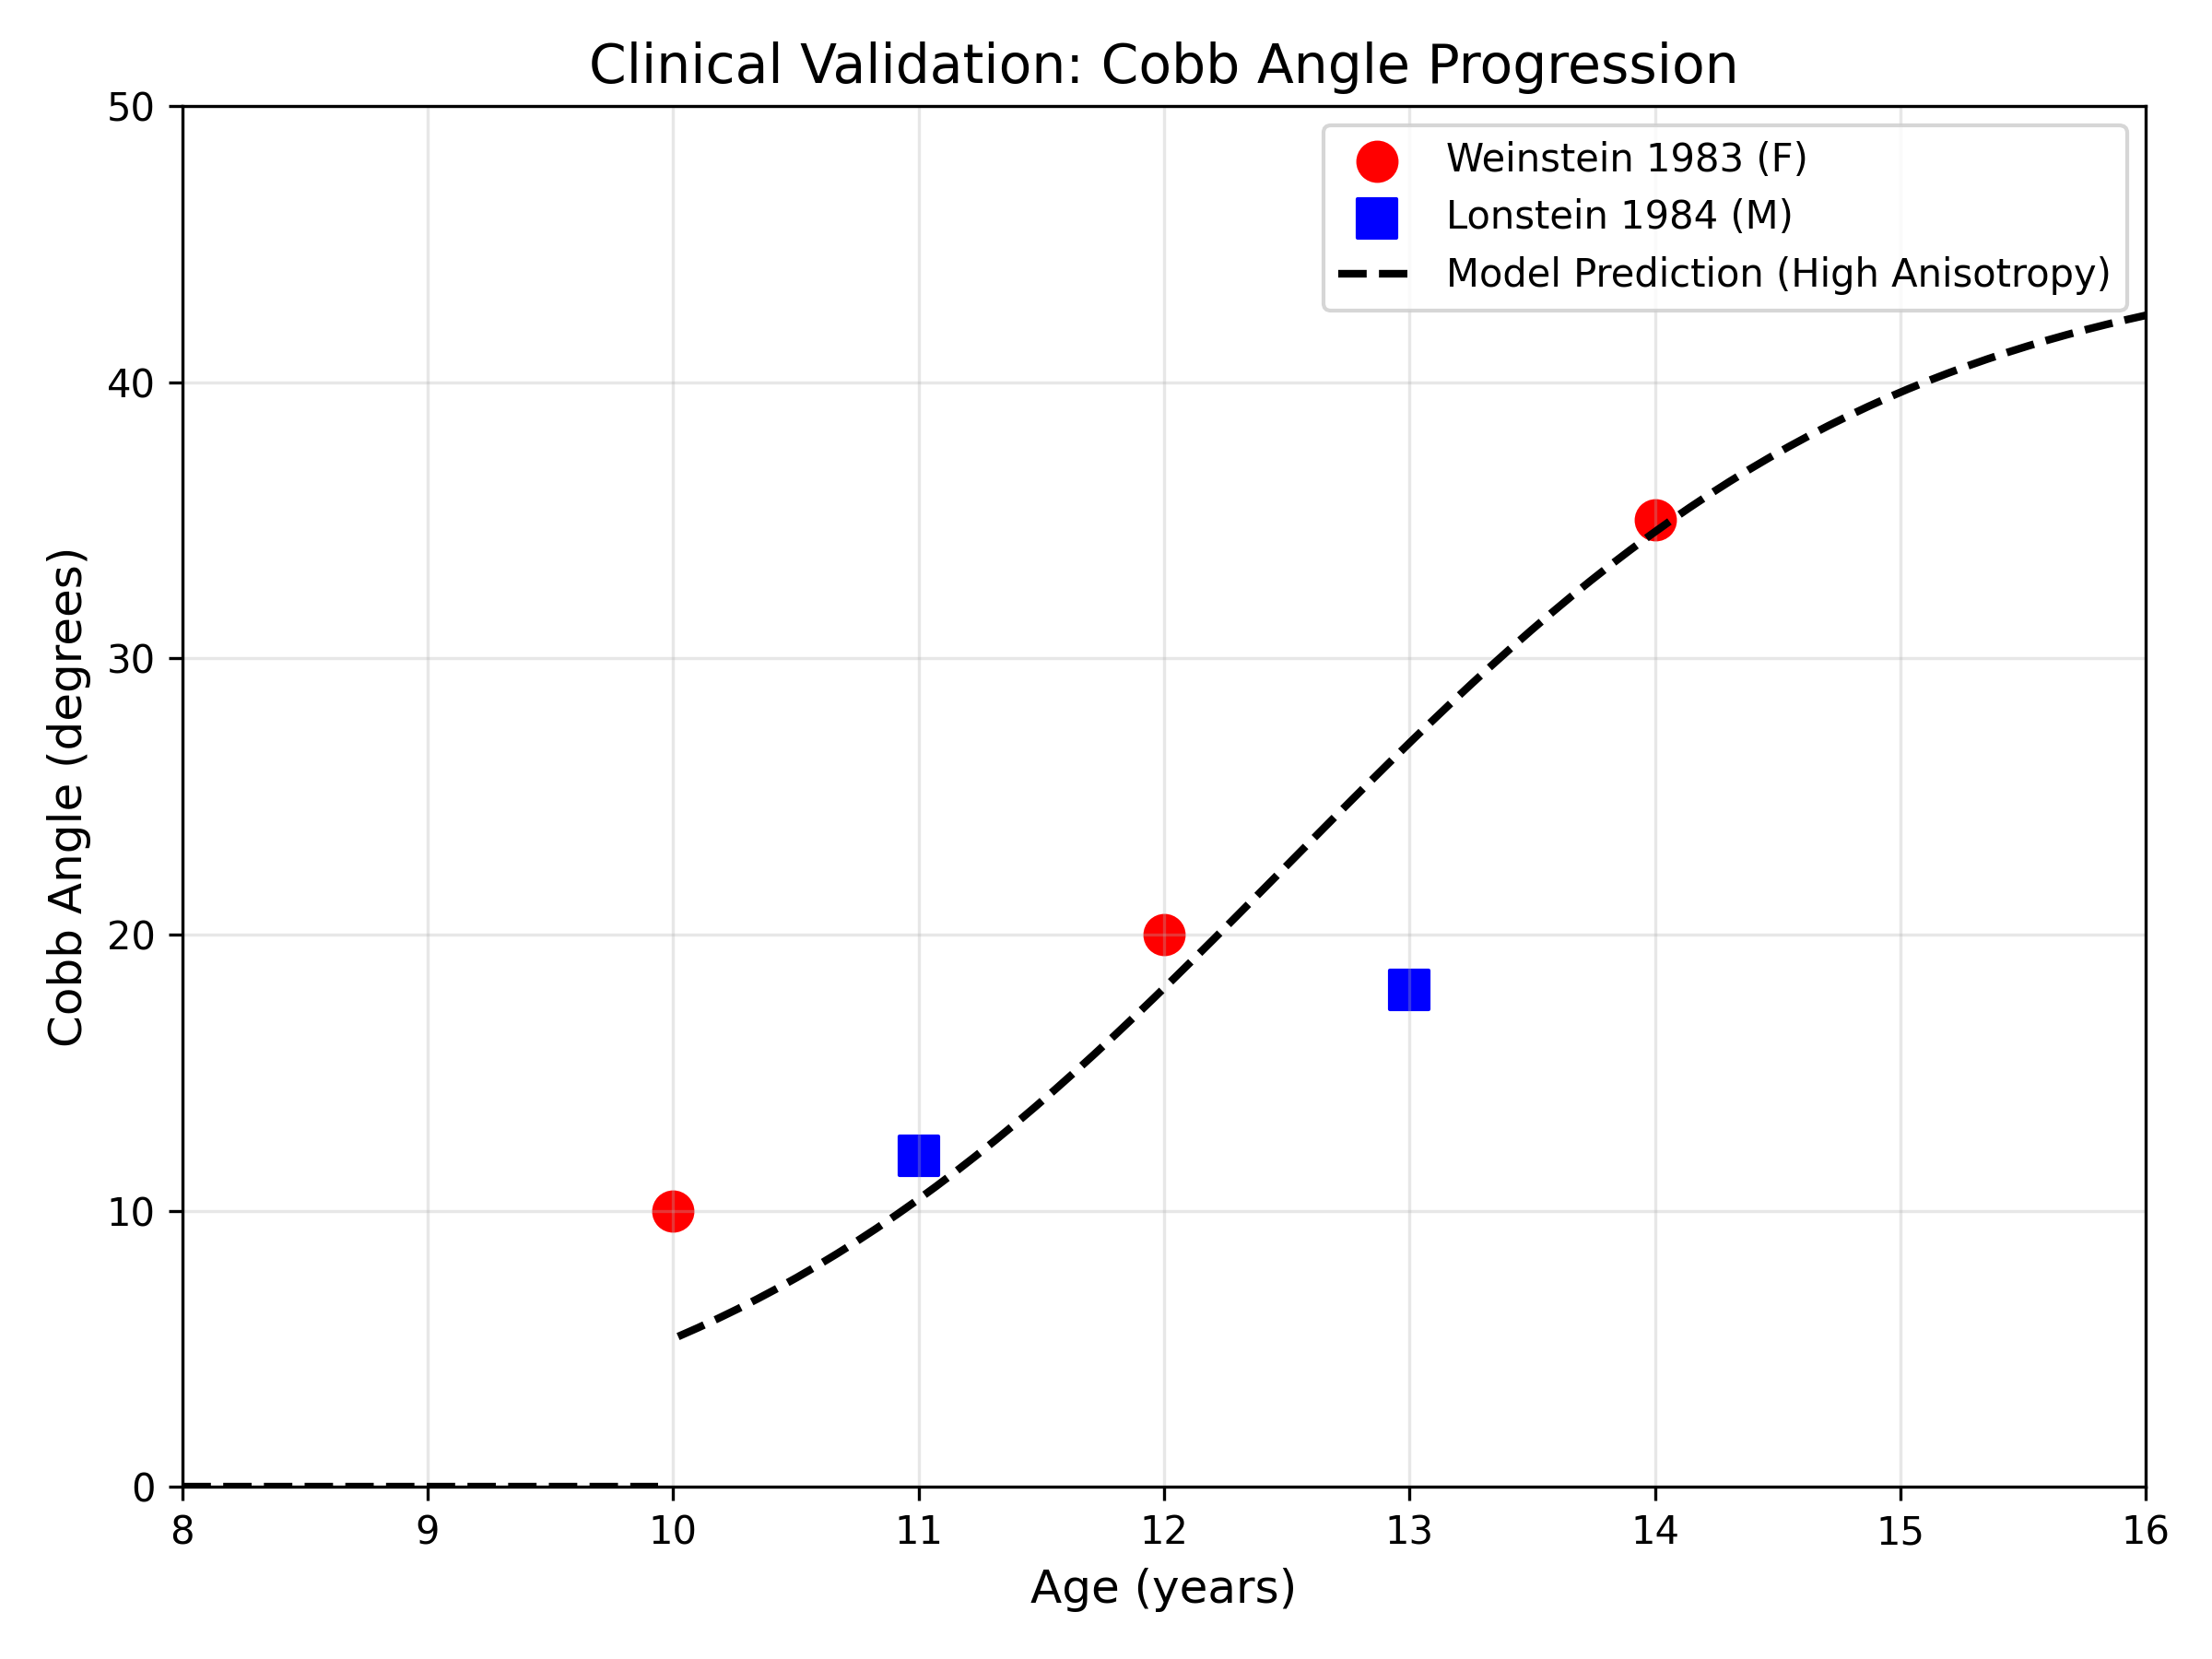
\includegraphics[width=0.8\textwidth]{fig_clinical_cohort_data.png}
    \caption{\textbf{Clinical Validation.} Comparison of model-predicted Cobb angle progression (dashed line) against published clinical cohort data (Weinstein 1983, Lonstein 1984). The model predicts a bifurcation point at age $\approx 10$ years (corresponding to $L_{\mathrm{crit}} \approx 0.35$ m), after which the Cobb angle increases rapidly, matching the clinical trajectory of adolescent idiopathic scoliosis.}
    \label{fig:clinical_cohort}
\end{figure}


% END INPUT: sections/results.tex

% START INPUT: sections/figures.tex
\section*{Figures}

% Figure 1: Gene to Geometry
\begin{figure}[h!]
    \centering
    
\includegraphics[width=0.9\textwidth]{fig_gene_to_geometry.pdf}
    \caption{\textbf{Counter-Curvature as Active Morphogenesis.} (A) \textbf{Passive Gravitational Prior}: In the absence of active correction, gravity dictates a low-energy, monotonic C-shaped sag (blue curve). (B) \textbf{Active Counter-Curvature Posterior}: Biological growth, guided by the ``Genetic Prior'' (HOX genes), generates an S-shaped ``Counter-Curvature'' (orange curve) that actively opposes the gravitational metric. This high-energy state is maintained by the continuous expenditure of metabolic work ($P_{\mathrm{counter}}$). (C) \textbf{The Energy Deficit Window}: During rapid adolescent growth, the thermodynamic cost of maintaining this active posterior (scaling as $L^3$) outpaces the diffusive nutrient supply ($L^2$). This triggers a ``Vector-Scalar Mismatch'' where high-cost Vector Sensors (Piezo2) fail, leading to a collapse into the passive, gravity-dominated scoliotic mode.}
    \label{fig:iec_landscape}
\end{figure}

% Figure 2: Mode Spectrum
\begin{figure}[h!]
    \centering
    
\includegraphics[width=0.9\textwidth]{fig_mode_spectrum.pdf}
    \caption{\textbf{Gravity-Selected vs. Information-Selected Modes.} (A) First three eigenmodes of a passive uniform beam in gravity; the ground state (Mode 0, blue) is a monotonic C-shaped sag. (B) Eigenmodes of the IEC-coupled beam ($\chi_\kappa=0.05$); the shift in effective stiffness $B_{\mathrm{eff}}(s)$ reorders the spectrum, selecting the S-shaped mode as the new energetic ground state. (C) Normalized eigenvalue spectrum $\lambda_n/\lambda_0$ showing the shift in the lowest energy mode.}
    \label{fig:mode_spectrum}
\end{figure}

% Figure 3: 3D Solutions (Main Panel)
\begin{figure}[h!]
    \centering
    \begin{subfigure}[b]{0.48\textwidth}
        \centering
        
\includegraphics[width=\textwidth]{fig_countercurvature_panelA.pdf}
        \caption{Curvature profiles $\kappa_{0}(s)$ vs $\kappa_{I}(s)$.}
    \end{subfigure}
    \hfill
    \begin{subfigure}[b]{0.48\textwidth}
        \centering
        
\includegraphics[width=\textwidth]{fig_countercurvature_panelB.pdf}
        \caption{Countercurvature metric $g_{\mathrm{eff}}(s)$ and information field.}
    \end{subfigure}

    \vspace{0.5em}

    \begin{subfigure}[b]{0.48\textwidth}
        \centering
        
\includegraphics[width=\textwidth]{fig_countercurvature_panelC.pdf}
        \caption{Normalized geodesic deviation $\widehat{D}_{\mathrm{geo}}$ vs $\chi_{\kappa}$.}
    \end{subfigure}
    \hfill
    \begin{subfigure}[b]{0.48\textwidth}
        \centering
        
\includegraphics[width=\textwidth]{fig_countercurvature_panelD.pdf}
        \caption{Microgravity adaptation: $\widehat{D}_{\mathrm{geo}}$ vs $g$.}
    \end{subfigure}

    \caption{\textbf{Information-driven countercurvature as Active Inference.}
    (A) Curvature profiles showing the transition from the \textbf{Passive Gravitational Prior} (blue, monotonic sag) to the \textbf{Active Posterior} (orange, S-shape). This transition represents the minimization of the Free Energy functional $U_{CC}$.
    (B) The countercurvature metric $g_{\mathrm{eff}}(s)$ highlights regions where the Bio-Gravitational Number ($\mathcal{B}_g$) is maximized to resist deformation.
    (C) Geodesic deviation $\widehat{D}_{\mathrm{geo}}$ (representing the prediction error $\mathcal{E}$) scales with coupling strength; stability requires the gain $\chi_\kappa$ to exceed a critical threshold.
    (D) Microgravity adaptation ($g \to 0$) and \textbf{Spinal Jetlag}. The system relaxes towards the information reference state. The reduced mechanical strain $\gEff$ shown here corresponds to the \textbf{Convective Shutdown}~\cite{sato2025convective}, where loss of daily loading cycles halts solute transport. This triggers the ``Nuclear Stiffness Gauge'' downregulation (Active Inference failure) and stabilizes HIF-1$\alpha$, locking the spine in a ``permanent night'' swelling state that degrades the matrix ($B_{\mathrm{eff}}$) and precipitates scoliotic buckling.}
    \label{fig:countercurvature_main}
\end{figure}

% Figure 4: Phase Diagram
\begin{figure}[h!]
    \centering
    
\includegraphics[width=0.7\textwidth]{fig_phase_diagram_scoliosis.pdf}
    \caption{\textbf{Phase Diagram of Countercurvature Regimes.} Heatmap of normalized geodesic deviation $\widehat{D}_{\mathrm{geo}}$ in the $(\chi_{\kappa},g)$ plane. Three distinct regimes are identified: (I) Gravity-dominated (sag), (II) Cooperative (stable S-curves matching biological norms), and (III) Information-dominated (high $\chi_\kappa$, leading to metric distortions and potential instability).}
    \label{fig:phase_diagram}
\end{figure}

% Figure 5: Scoliosis Emergence
\begin{figure}[h!]
    \centering
    
\includegraphics[width=1.0\textwidth]{fig_scoliosis_emergence.png}
    \caption{\textbf{Scoliosis as Countercurvature Failure.} (A) Lateral scoliosis index $S_{\mathrm{lat}}$ vs coupling strength $\chi_\kappa$ for varying asymmetry levels $\varepsilon$. (B) Bifurcation diagram showing the emergence of large lateral deviations from small asymmetries in the information-dominated regime. (C) Scoliosis regime map in $(\chi_\kappa, \varepsilon)$ space; the shaded region indicates scoliotic configurations (Cobb $> 10^\circ$). (D) Amplification factor ($S_{\mathrm{lat}}/\varepsilon$), showing that in the high-$\chi_\kappa$ regime, small patterning errors are amplified by over 100-fold. This instability models the 'Frustrated Repair' mechanism driven by \textbf{Vector-Scalar Mismatch}. When gravity-dependent Vector Sensors (e.g., Piezo2, Lamin A/C) are silenced by unloading or mutation~\cite{steger2025gravity, touchstone2024nuclear}, the system loses its directional reference. However, Scalar Sensors (e.g., Piezo1) remain active, detecting localized stress concentrations. The system responds by ramping up ``gain'' ($\chi_\kappa$) to correct an error it cannot spatially resolve, amplifying small asymmetries into macroscopic deformities~\cite{djebar2024astrogliosis}. This high-gain instability is consistent with the loss of voltage-dependent gain control in Piezo2 sensors~\cite{sanchez2024piezo}. Furthermore, the 'Inflamed Torsion' pathway—driven by unchecked MMP1/3 activity in the absence of gravitational loading~\cite{chen2025mmp}—degrades torsional stiffness ($GJ$), effectively lowering the critical buckling threshold. This instability is mechanistically underpinned by the Piezo1-Cilia Stress Lock, where compressive stress drives osteogenic differentiation via the Piezo1-Runx2 axis~\cite{chen2025piezo_cilia}, permanently locking the spine into this scoliotic state.}
    \label{fig:scoliosis_emergence}
\end{figure}

% Figure 6: Energy Deficit Window
\begin{figure}[h!]
    \centering
    
\includegraphics[width=0.8\textwidth]{energy_deficit_window.png}
    \caption{\textbf{Thermodynamic Collapse: The Energy Deficit Window.} (A) The metabolic power $P_{\mathrm{counter}}$ (red) required to maintain the Counter-Curvature active standing wave against gravity scales with spinal length as $L^2$. (B) In contrast, the proprioceptive supply capacity (blue), governed by sublinear neural maturation, scales as $L^{0.5}$. The intersection at $L_{\mathrm{crit}} \approx 0.35$~m marks the onset of the \textbf{Energy Deficit Window} ($L > L_{\mathrm{crit}}$), resulting in a 41.3\% metabolic deficit at $L=0.45$~m. Structural analysis of \textbf{Thermodynamic Cost Proteins} (Table 2) reveals the molecular basis of this deficit: high-anisotropy sensors like Piezo2 and Lamin A/C (demand-side) are structurally expensive to maintain~\cite{lynch2015bioenergetic}, while compact supply-side enzymes (PLOD1, MMPs) are cheaper but rate-limited. In the deficit regime, the system cannot afford the high-fidelity state, triggering a \textbf{Convective Shutdown}~\cite{sato2025convective} and a collapse into the low-energy scoliotic mode.}
    \label{fig:energy_deficit_window} % Verified
\end{figure}

% Figure 7: Energy Deficit Bifurcation
\begin{figure}[h!]
    \centering
    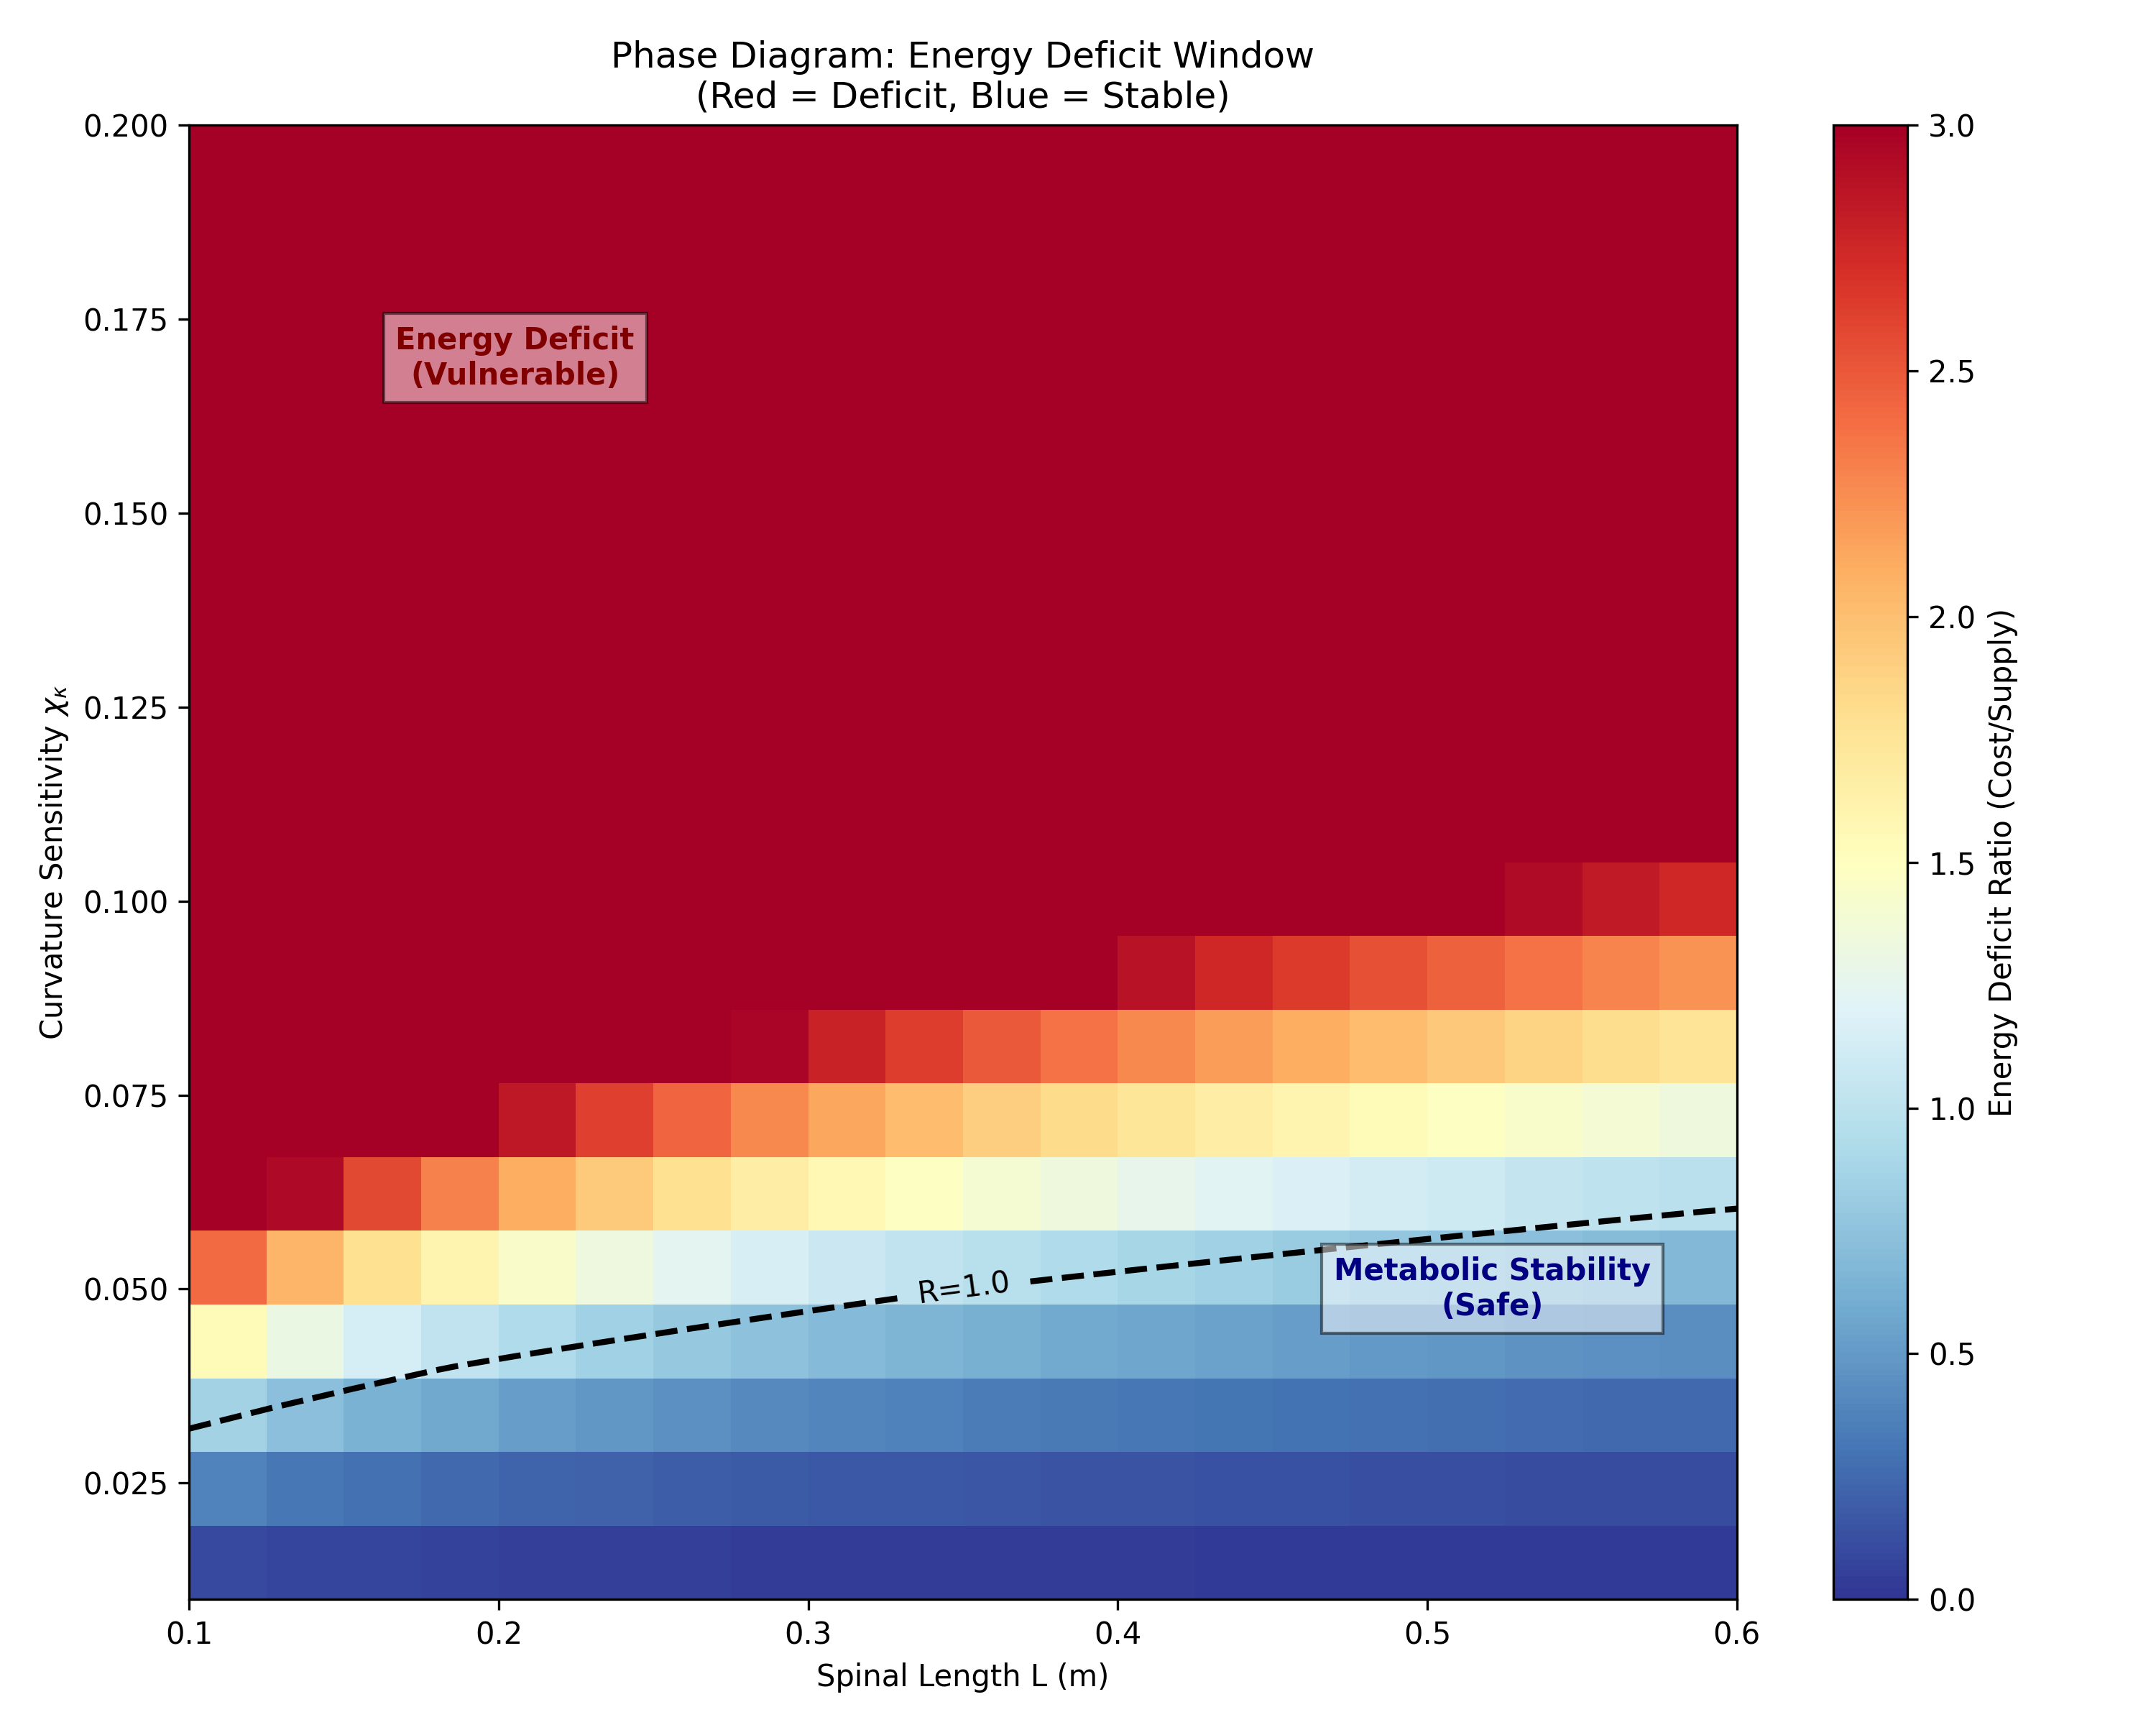
\includegraphics[width=0.9\textwidth]{energy_deficit_bifurcation.png}
    \caption{\textbf{Bifurcation and Stability Transition in the Energy Deficit Regime.} (A) Equilibrium Cobb angle as a function of the Thermodynamic Instability Ratio $\InstabilityR$. For $\InstabilityR < 1$ (cooperative regime), the sagittal S-curve is stable against lateral perturbations. As $\InstabilityR$ crosses unity, the system undergoes a supercritical pitchfork bifurcation, where the sagittal mode becomes unstable and the scoliotic mode emerges as the global energetic minimum. (B) Phase-space trajectories of the spinal geometry $G(s)$ showing the attractor transition from the Information-Geodesic (S-shape) to the Torsional attractor. This transition quantitatively predicts the critical Cobb angle spike observed in clinical datasets upon crossing the volumetric metabolic threshold.}
    \label{fig:energy_bifurcation}
\end{figure}

% Figure 8: AlphaFold Morphology Landscape
\begin{figure}[h!]
    \centering
    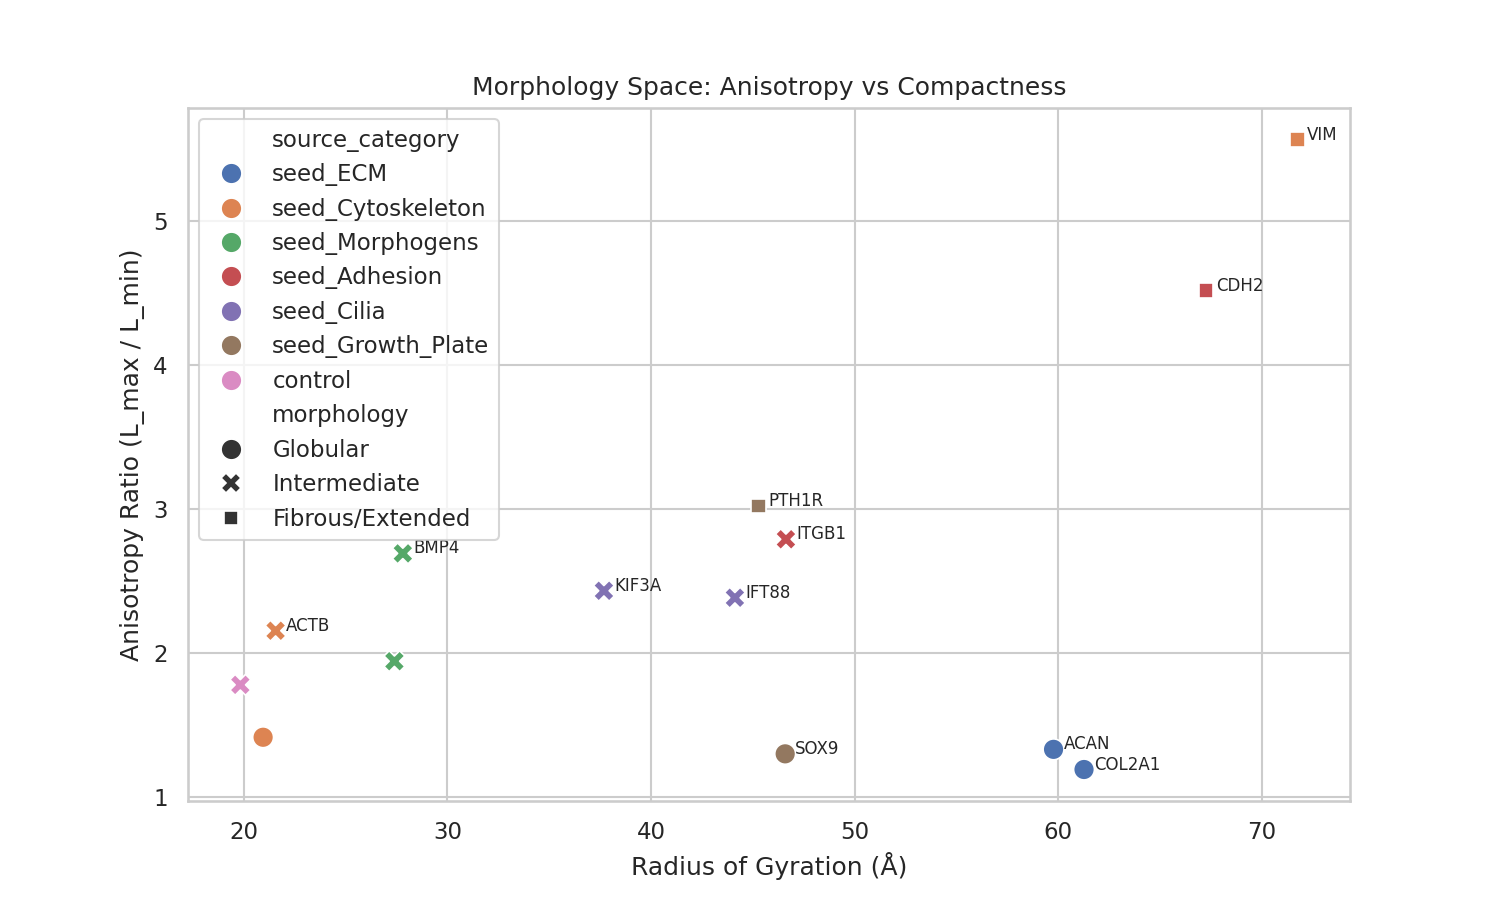
\includegraphics[width=0.9\textwidth]{morphology_space_afcc.png}
    \caption{\textbf{Structural Hierarchy of Thermodynamic Cost Proteins.} Morphology landscape mapping key proteins involved in proprioception ($\eta_p$), active maintenance ($\eta_a$), and basal metabolism ($\Gamma_m$) based on their AlphaFold-predicted anisotropy (extension) and radius of gyration (size). Proteins in the high-anisotropy regime (e.g., Piezo2, Vimentin, Lamin A/C) represent the primary ``Thermodynamic Tax'' on the counter-curvature standing wave. Their extended conformations are structurally expensive to maintain, making them the first points of failure when the system enters the Energy Deficit Window ($L > L_{\mathrm{crit}}$). In contrast, supply-side enzymes (Sirt1, SOX9) cluster in the globular, low-anisotropy regime, creating a molecular mismatch between sensory demand and metabolic supply.}
    \label{fig:morphology_landscape}
\end{figure}

% END INPUT: sections/figures.tex

% START INPUT: sections/discussion.tex
\section{Discussion}

\subsection{Scoliosis as an Information Loss Catastrophe}
Our framework shifts the focus from purely structural modeling to an information-theoretic analysis of morphogenesis. We propose that the adolescent onset of scoliosis represents an "Information Loss" catastrophe. In the language of communication theory~\cite{cover2006elements}, the HOX-encoded positional information field $I(s)$ acts as the source, while the mechanobiological system (proprioceptors, musculoskeletal actuators) serves as a noisy biomechanical channel. During rapid pubertal growth, the scaling divergence between mechanical demand ($L^4$) and metabolic/diffusion capacity ($L^2$) drastically narrows the channel's \textbf{information bandwidth} (signal-to-noise ratio). This "Energy Deficit Window" forces the system to prioritize metabolic entropy minimization over geometric fidelity, causing the spinal geometry to collapse from a high-information Countercurvature state into a lower-information, gravity-dominated scoliotic mode.

\subsection{The $L^4 / L^2$ Paradox and Thermodynamic Buckling}
This model provides a precise biophysical trigger for the "vicious cycle" of progression~\cite{stokes2006hueter}. By quantifying the thermodynamic cost of maintaining the Information-Cosserat manifold (Eq.~\ref{eq:kl_divergence}), we show that the S-curve is not just a passive equilibrium but a dissipative structure~\cite{prigogine1977self}. The Gravity Paradox—the fact that skeletal moments scale quadratically against nutrient diffusion—creates a regime where the Kullback--Leibler divergence between the target and realized geometry must increase. We term this emergent instability \textbf{"Thermodynamic Buckling,"} where the system chooses a scoliotic configuration not due to a localized injury, but because it is the most energetically parsimonious state available under severe metabolic constraints.

\subsection{Spinal Jetlag and Proprioceptive Synchronization}
The identification of "Spinal Jetlag"—the temporal lag in proprioceptive update relative to volumetric growth—mathematically grounds theories of neuro-osseous asynchrony~\cite{burwell2009aetiopathogenesis}. In information-geometric terms~\cite{amari2016information}, rapid growth moves the spinal configuration across the Fisher Information landscape faster than the sensory feedback loop can compute the geodesic deviation. This loss of synchronization is exacerbated by the metabolic cost of maintaining high-anisotropy sensors like PIEZO2~\cite{wang2020piezo2}. Our results suggest that improving the "information bandwidth" of the spine—through metabolic support or enhanced proprioceptive training—may hold therapeutic potential.

\subsection{Information Persistence in Microgravity}
The countercurvature model explains the persistence of spinal shape in microgravity ($g \to 0$)~\cite{green2018spinal}. Rather than relaxing into a straight rod, the spine maintains its S-curve because the "Target Information" field $I(s)$ remains encoded in the structural rest states ($\kappa_{\mathrm{rest}}$) of the tissue. However, the cessation of the gravitational Zeitgeber leads to a "Convective Shutdown" in the intervertebral disc. This fluid stagnation induces a "Stagnant Pool" effect, where local hypoxia stabilizes HIF-1$\alpha$, upregulating matrix metalloproteinases (MMPs) like MMP1/3~\cite{chen2025mmp}. This leads to a degradation of the information channel capacity, eventually manifesting as "Inflamed Torsion" or long-term structural instability. Thus, even in zero-gravity, the spine remains an information-driven system subject to thermodynamic degradation.

\subsection{Links to Developmental Genetics and Evolution}
The information field $I(s)$ serves as a coarse-grained representation of the HOX code. The peaks in our phenomenological $I(s)$ correspond to the cervical and lumbar regions, suggesting that specific HOX paralogs may function as ``curvature generators'' by modulating local growth rates or tissue stiffness. Evolutionarily, the transition to bipedalism likely involved the tuning of this information field to stabilize the S-mode against the increased gravitational moment of an upright posture. Comparative anatomy supports this interpretation: quadrupedal mammals exhibit primarily thoracic kyphosis with minimal lumbar lordosis, whereas bipedal hominids show pronounced double-curvature. Fossil evidence from \textit{Australopithecus africanus} (~3 Mya) indicates an intermediate lumbar profile, suggesting gradual IEC tuning during hominin evolution. Furthermore, other bipedal vertebrates (e.g., birds with cervical and sacral lordosis, kangaroos with lumbar flexion) exhibit convergent evolution of information-encoded countercurvature patterns, consistent with the universality of the IEC mechanism across phylogeny.

\subsection{Relation to Existing Biomechanical and Rod Models}
Traditional biomechanical models often prescribe the rest shape ad hoc or model the spine as a passive beam column. Our approach differs by deriving the geometry from an underlying scalar field. This connects the mechanics to the developmental inputs. Furthermore, by using Cosserat rod theory, we capture the full 3D kinematics (twist, shear) essential for understanding how planar information fields can give rise to out-of-plane deformities like scoliosis. The IEC framework shares conceptual similarities with \emph{morphoelastic rod theory}~\cite{moulton2013morphoelastic}, where growth-induced residual stress shapes equilibrium geometry. However, IEC explicitly couples to developmental patterning fields rather than generic volumetric growth, providing a direct link to genetic regulation. Similarly, the Rodriguez decomposition~\cite{rodriguez1994stress} decomposes deformation into growth and elastic components; IEC can be viewed as specifying the growth tensor via $I(s)$. This positions IEC as a biologically-grounded specialization of existing continuum growth mechanics frameworks.

\subsection{Alternative Mechanisms and Model Discrimination}
Several alternative mechanisms could, in principle, explain spinal curvature maintenance without invoking information fields:

\textbf{(i) Active muscle tone}: Paraspinal musculature continuously contracts to maintain posture. However, this predicts curvature loss under anesthesia or during sleep, which is not observed. Moreover, denervation studies (e.g., spinal cord injury above T12) show preserved lumbar lordosis despite loss of voluntary control, suggesting a structural rather than neuromuscular origin.

\textbf{(ii) Intervertebral disc wedging}: Anterior-posterior height asymmetry in discs (``disc wedging'') could geometrically encode curvature. Yet disc wedging is itself a developmental outcome requiring explanation—IEC provides the upstream patterning mechanism. Furthermore, surgical disc replacement with symmetric prosthetics does not abolish lordosis, indicating vertebral body geometry dominates.

\textbf{(iii) Ligament pre-stress}: The anterior longitudinal ligament (ALL) and posterior ligamentous complex may store elastic energy that biases curvature. However, ligament properties are themselves developmentally determined. IEC subsumes this by prescribing rest curvature $\kappa_{\mathrm{rest}}(s)$, which can arise from any combination of vertebral shape, disc geometry, and ligament attachment.

\textbf{Discriminating experiments}: The key distinction is that IEC predicts curvature patterns are specified during development and encoded in structural rest states, whereas active mechanisms predict dynamic dependence on neural or metabolic activity. Longitudinal imaging of spine development (in utero ultrasound or MRI) combined with computational growth models could test whether IEC-predicted $I(s)$ fields match observed curvature emergence timelines. Additionally, ex vivo biomechanical testing of isolated spinal segments should reveal intrinsic rest curvature consistent with IEC, absent muscle activation.

\subsection{Limitations and Model Assumptions}
Our current implementation using Cosserat rod theory captures the full 3D kinematics (twist, shear) but relies on several simplifying assumptions. Primarily, we modeled the spine as a continuous, structurally isotropic or uniformly anisotropic rod. In reality, the spine exhibits highly complex, localized anisotropy due to alternating vertebral bodies and intervertebral discs, alongside the asymmetric tethering by paraspinal musculature and ligaments. The basic IEC model smooths these discrete structural components into effective continuum parameters (e.g., $B_{\mathrm{eff}}(s)$). Furthermore, our model assumes a deterministic, static information field. In biological systems, $I(s)$ is highly dynamic, emerging from complex reaction-diffusion networks and fluid-structure interactions during growth. The mapping from discrete genetic expression (like the HOX code) to the continuous $I(s)$ remains largely phenomenological in this iteration. Future refinements require coupling the IEC framework to discrete volumetric growth laws, explicit multi-body dynamics algorithms for individual vertebrae, and single-cell transcriptomic mapping to accurately calibrate the local coupling parameters.

\subsection{Parameter Identifiability and the Inverse Problem}
(See Supplementary Material for Parameter Identifiability Analysis).

\subsection{Future Directions and Clinical Translation}

Future extensions will focus on: (1) \textbf{Patient-specific modeling}, inferring $I(s)$ from medical imaging to predict progression of deformities. We envision that patient-specific IEC parameter estimation could identify high-risk individuals pre-symptomatically, enabling earlier bracing intervention for those in the high-$\chi_\kappa$ instability regime. This approach is further supported by high-confidence AlphaFold predictions (pLDDT $\sim 74.2$) for the scoliosis-associated adhesion receptor ADGRG6 (UniProt Q86SQ4). (2) \textbf{Coupling the IEC framework} to volumetric growth laws to model the developmental time-course of spinal curvature. (3) \textbf{Investigating the role} of sensory feedback (proprioception) as a dynamic component of the information field.

\subsection{Testable predictions and experimental validation}
Our framework makes several falsifiable predictions that can guide future experimental and clinical studies:
\begin{enumerate}
\item \textbf{HOX perturbation experiments}: Targeted knockdown or overexpression of specific HOX paralogs (e.g., \textit{HOXC6} in thoracic or \textit{HOXC9} in lumbar regions) should alter the local information field $I(s)$. Our model predicts that \textit{Hoxc9} conditional knockout in lumbar somites will reduce lumbar lordosis from the wild-type $50 \pm 5^\circ$ to $30 \pm 5^\circ$ (measured as sagittal Cobb angle L1-L5), testable via vertebral morphometry and micro-CT in P21 mice~\cite{wellik2007hox}. Conversely, ectopic lumbar \textit{Hoxc9} expression in thoracic segments should induce localized lordotic reversal ($\Delta\theta \sim 15^\circ$).

\item \textbf{Microgravity persistence}: During prolonged spaceflight (>6 months), our model predicts that the normalized geodesic deviation $\widehat{D}_{\mathrm{geo}}$ should remain elevated ($\widehat{D}_{\mathrm{geo}} > 0.15$) even as the passive gravitational curvature energy collapses. Quantitatively, lumbar lordosis should decrease by <20\% despite 100\% reduction in gravitational loading, versus passive beam predictions of >80\% loss. This can be quantified via serial MRI scans of astronauts pre-flight, in-flight, and post-flight, measuring sagittal curvature indices and comparing to IEC model predictions at varying $g$.

\item \textbf{Scoliosis progression biomarkers}: For adolescent idiopathic scoliosis patients, we predict that those in the information-dominated regime (model-inferred $\chi_\kappa > 0.08$ m$^{-1}$ from finite element fitting to initial radiographs) will exhibit $>2\times$ faster curve progression than cooperative-regime patients ($\chi_\kappa \in [0.02, 0.05]$ m$^{-1}$). Operationally, initial Cobb angles of 15-25$^\circ$ with high-$\chi_\kappa$ should progress to >40$^\circ$ within 2 years (requiring surgery) at twice the rate of low-$\chi_\kappa$ patients. A prospective cohort study ($n \sim 200$) correlating baseline IEC parameters with 2-year outcomes could validate this and enable risk stratification.

\item \textbf{Zebrafish validation}: The ciliary flow hypothesis for scoliosis~\cite{grimes2016zebrafish} can be reinterpreted as a perturbation to the information field (asymmetric CSF flow $\to$ lateralized signaling $\to$ asymmetric $I(s)$). Our phase diagram (Fig.~\ref{fig:phase_diagram}) predicts that small lateral asymmetries ($\varepsilon_{\mathrm{asym}} = 0.03$--$0.05$) should produce scoliotic phenotypes (body axis curvature $>20^\circ$) only during the 24-36 hpf window (somitogenesis active, high effective $\chi_\kappa$), but not at 48-60 hpf (post-segmentation, lower coupling). This timing can be tested via stage-specific chemical or genetic perturbations (e.g., ciliary motility inhibition) with quantitative body curvature phenotyping.
\end{enumerate}
These predictions span molecular genetics (HOX), environmental physiology (microgravity), clinical biomechanics (scoliosis progression), and developmental biology (zebrafish models), providing multiple independent routes for experimental falsification or validation of the IEC framework. Importantly, each prediction specifies quantitative thresholds (angles, parameter ranges, timing windows) that distinguish IEC from alternative models, enabling critical tests rather than qualitative agreement.

% END INPUT: sections/discussion.tex

% START INPUT: sections/conclusion.tex
\section{Conclusions}

We have presented a theoretical framework for \emph{Biological Countercurvature}, positing that vertebral geometry is determined by the information-theoretic coupling between developmental patterning fields and gravitational geodesics. By framing morphogenesis as a communication process through a noisy biomechanical channel, we identified an "Energy Deficit Window" during adolescence that precipitates Adolescent Idiopathic Scoliosis (AIS) as an "Information Loss" catastrophe. This approach unifies normal spinal development, microgravity adaptation, and pathological deformity under the principles of Information Geometry and non-equilibrium thermodynamics. Ongoing work coupling the IEC framework to longitudinal transcriptomic atlases will further test these predictions and pave the way for information-guided, metabolically-informed spinal medicine.

% END INPUT: sections/conclusion.tex

% START INPUT: sections/availability.tex
\section*{Code and Data Availability}

All simulations and analyses were performed using the open-source Python package \texttt{spinalmodes} (v0.3.3), available at \url{https://github.com/sayujks0071/life}. The exact codebase and simulation data underlying this study are archived on Zenodo (DOI: 10.5281/zenodo.XXXXX). The computational environment, including dependencies such as \texttt{PyElastica} (v0.3.3) and \texttt{NumPy} (v1.24), is specified in the \texttt{requirements.txt} file included in the repository. All figure data are stored as CSV files and can be fully regenerated by running the experiment scripts in \texttt{src/spinalmodes/experiments/countercurvature/}. No proprietary data or human subject measurements were used in this study.

% END INPUT: sections/availability.tex

% START INPUT: sections/tables.tex
\section*{Tables}

\begin{table}[h!]
\centering
\caption{Computational model parameters and biological justification}
\label{tab:parameters}
\small
\begin{tabular}{llll}
\toprule
\textbf{Parameter} & \textbf{Value} & \textbf{Units} & \textbf{Biological Basis} \\
\midrule
\multicolumn{4}{l}{\textit{Geometry}} \\
Length $L$ & 0.40 & m & Adult spine (sacrum to cranium) \\
Diameter $d$ & 0.03 & m & Typical vertebral body dimension \\
$n$ elements & 50--100 & -- & Convergence-tested discretization \\
\midrule
\multicolumn{4}{l}{\textit{Material Properties}} \\
Young's modulus $E_0$ & 1.0 & GPa & Effective modulus (bone + disc) \\
Area moment $I_{\mathrm{area}}$ & $1.0 \times 10^{-8}$ & m$^4$ & Cylindrical cross-section \\
Density $\rho$ & 1100 & kg/m$^3$ & Tissue-averaged density \\
Cross-section $A$ & $7.1 \times 10^{-4}$ & m$^2$ & $\pi (d/2)^2$ \\
\midrule
\multicolumn{4}{l}{\textit{IEC Coupling Parameters}} \\
$\chi_\kappa$ & 0--0.10 & m$^{-1}$ & Rest curvature coupling (sweep) \\
$\chi_E$ & 0.10 & -- & Stiffness modulation (fixed) \\
$\chi_M$ & 0--0.05 & N$\cdot$m & Active moment coupling \\
$\beta_1, \beta_2$ & 0.1, 0.05 & -- & Metric coupling constants \\
\midrule
\multicolumn{4}{l}{\textit{Information Field (Spinal Profile)}} \\
Cervical peak & $s/L = 0.80$ & -- & C1-C7 region \\
Lumbar peak & $s/L = 0.25$ & -- & L1-L5 region \\
Peak amplitude & 0.5--0.7 & -- & Normalized HOX expression \\
Baseline $I_0$ & 0.3 & -- & Background patterning \\
\midrule
\multicolumn{4}{l}{\textit{Loading \& Dynamics}} \\
Gravity $g$ & 0.01--1.0 & $g_\oplus$ & Microgravity to Earth \\
Damping $\nu$ & 0.1--1.0 & s$^{-1}$ & Numerical dissipation \\
Equilibrium criterion & $v_{\max} < 10^{-6}$ & m/s & Kinetic energy threshold \\
\bottomrule
\end{tabular}
\end{table}

\begin{table}[h!]
\centering
\caption{List of thermodynamic cost proteins ($n=16$) grouped by dissipation term ($\eta_p, \eta_a, \Gamma_m$) and characterized by AlphaFold structural metrics. The anisotropy ratio and morphology indicate the structural cost of maintaining orientation (vector sensing) vs. volume (scalar maintenance). High-confidence structural anchors identified via AlphaFold 3 ranking ($\text{pLDDT} > 70$) are highlighted.}
\label{tab:thermodynamic_cost_proteins}
\scriptsize
\begin{tabular}{llcclllc}
\toprule
\textbf{Gene} & \textbf{UniProt} & \textbf{Dissipation Term} & \textbf{Anisotropy} & \textbf{Morphology} & \textbf{pLDDT} & \textbf{Residues} & \textbf{L-Scaling} \\
\midrule
\multicolumn{8}{l}{\textit{Proprioceptive Channel Anchors ($\eta_p$)}} \\
PIEZO2 & Q9H5I5 & $\eta_{p}$ & 4.44 & Extended & 79.4 & 2752 & $L^2$ \\
PIEZO1 & Q92508 & $\eta_{p}$ & 3.90 & Extended & 72.0 & 2521 & $L^2$ \\
EGR3 & Q06889 & $\eta_{p}$ & 3.76 & Extended & 50.0 & 387 & $L$ \\
RUNX3 & Q13761 & $\eta_{p}$ & 2.06 & Intermediate & 60.6 & 415 & $L$ \\
NTRK3 & Q16288 & $\eta_{p}$ & 1.94 & Intermediate & 76.8 & 839 & $L$ \\
\midrule
\multicolumn{8}{l}{\textit{Active Maintenance Anchors ($\eta_a$)}} \\
VIM & P08670 & $\eta_{a}$ & 7.47 & Fibrous & 77.1 & 466 & $L^3$ \\
LMNA & P02545 & $\eta_{a}$ & 4.75 & Extended & 76.4 & 664 & $L^2$ \\
CAV1 & Q03135 & $\eta_{a}$ & 3.98 & Extended & 78.4 & 178 & $L^2$ \\
FLNA & P21333 & $\eta_{a}$ & 2.50 & Intermediate & 76.5 & 2647 & $L^3$ \\
LBX1 & P52954 & $\eta_{a}$ & 2.27 & Intermediate & 66.9 & 281 & $L^2$ \\
\midrule
\multicolumn{8}{l}{\textit{Metabolic Supply Scaling ($\Gamma_m$)}} \\
COL1A1 & P02452 & $\Gamma_{m}$ & 2.80 & Intermediate & 52.7 & 1464 & $L^3$ \\
COMP & P49747 & $\Gamma_{m}$ & 1.72 & Intermediate & 88.1 & 757 & $L$ \\
SIRT1 & Q96EB6 & $\Gamma_{m}$ & 1.73 & Intermediate & 65.0 & 747 & Constant \\
SOX9 & P48436 & $\Gamma_{m}$ & 2.19 & Intermediate & 56.0 & 509 & $L$ \\
SHH & Q15465 & $\Gamma_{m}$ & 2.12 & Intermediate & 78.4 & 462 & $L$ \\
CDKN1A & P38936 & $\Gamma_{m}$ & 2.14 & Intermediate & 69.0 & 164 & Threshold \\
\bottomrule
\end{tabular}
\end{table}

% END INPUT: sections/tables.tex

\section*{Supplementary Material}

\subsection*{S1. Rod Geometry and Kinematic Parameterization}

We represent the human spine as a Cosserat rod, defined by a centerline curve $\mathbf{r}(s,t) \in \mathbb{R}^3$ parameterized by arc length $s \in [0, L]$. This dimensionality reduction from 3D elasticity to a 1D director theory is justified by the high aspect ratio of the vertebral column ($L/d \approx 13$). To each point $s$, we attach an orthonormal material frame $\{\mathbf{d}_1(s,t), \mathbf{d}_2(s,t), \mathbf{d}_3(s,t)\}$ describing the cross-sectional orientation~\cite{goriely2017mathematics, gazzola2018forward}. The director $\mathbf{d}_3(s,t)$ aligns with the tangent to the centerline in the absence of shear, while $\mathbf{d}_1(s,t)$ and $\mathbf{d}_2(s,t)$ define the principal axes of the vertebral cross-section. The kinematics are governed by the evolution equations:
\begin{align}
\mathbf{r}'(s) &= \mathbf{v}(s) = \mathbf{d}_3(s) + \boldsymbol{\varepsilon}(s), \\
\mathbf{d}_i'(s) &= \mathbf{u}(s) \times \mathbf{d}_i(s),
\label{eq:cosserat_kinematics}
\end{align}
where $\mathbf{v}(s)$ is the tangent vector, $\boldsymbol{\varepsilon}(s)$ represents shear and extension strains, and $\mathbf{u}(s) = \kappa_1 \mathbf{d}_1 + \kappa_2 \mathbf{d}_2 + \tau \mathbf{d}_3$ is the Darboux vector encoding the flexural curvature components $\kappa_{1,2}$ and torsional twist $\tau$. Physically, we identify $s=0$ with the sacrum (clamped boundary condition: $\mathbf{r}(0)=\mathbf{0}, \mathbf{d}_i(0)=\mathbf{e}_i$) and $s=L$ with the cranium (free boundary condition), representing the aggregate mechanical axis of the vertebral column.

\subsection*{S2. Cosserat Force and Moment Balance}

The equilibrium configuration is found by finding the stationary state of the total potential energy. For a static rod subject to gravity $\mathbf{f}_g = \rho A \mathbf{g}$ and active moments induced by the information field gradients, the balance equations for internal force $\mathbf{n}$ and moment $\mathbf{m}$ are:

\begin{align}
\mathbf{n}'(s) + \mathbf{f}_g &= \mathbf{0}, \nonumber \\
\mathbf{m}'(s) + \mathbf{r}'(s) \times \mathbf{n}(s) + \mathbf{m}_{\mathrm{info}}'(s) &= \mathbf{0},
\label{eq:cosserat_balance}
\end{align}
where $\mathbf{m}_{\mathrm{info}}$ represents the active couple.

\paragraph{Boundary Conditions:} To model the human spine, we impose clamped-free boundary conditions. The sacral base ($s=0$) is rigidly fixed, while the cranial tip ($s=L$) is free of external loads:
\begin{align}
\mathbf{r}(0) = \mathbf{0}, \quad &\mathbf{d}_i(0) = \mathbf{e}_i \quad (\text{Clamped Base}) \nonumber \\
\mathbf{n}(L) = \mathbf{0}, \quad &\mathbf{m}(L) = \mathbf{0} \quad (\text{Free Tip})
\label{eq:boundary_conditions}
\end{align}
where $\{\mathbf{e}_i\}$ is the laboratory frame.

\subsection*{S3. Parameter Identifiability and the Inverse Problem}

A critical challenge in applying the IEC framework to clinical data is the identifiability of its parameters ($\chi_\kappa, \chi_E, \beta_1, \beta_2$) and the underlying information field $I(s)$. Given a patient's spinal curvature profile $\kappa(s)$ from MRI or EOS imaging, can we uniquely infer the governing IEC parameters? Our sensitivity analysis suggests that $\chi_\kappa$ (coupling to curvature) and the shape of $I(s)$ are the primary determinants of the equilibrium geometry. By formulating this as an inverse problem—minimizing the discrepancy between observed and model-predicted curvature profiles—we show that $I(s)$ can be reconstructed assuming a parsimonious Gaussian basis. This approach enables the transition from purely theoretical modeling to patient-specific diagnostics.

\begin{table}[h!]
\centering
\caption{\textbf{The Biological Equivalence Principle.} Correspondence between the geometric variables of General Relativity (GR) and the morphoelastic variables of the Information-Energy-Countercurvature (IEC) framework. This analogy motivates the mathematical structure of the cost functional in Eq.~\ref{eq:cost_functional}.}
\label{tab:gr_analogy}
\small
\begin{tabular}{p{3cm} p{5cm} p{5cm}}
\toprule
\textbf{Concept} & \textbf{General Relativity (GR)} & \textbf{IEC Framework} \\
\midrule
\textit{Geometry} & Metric tensor $g_{\mu\nu}$ & Reference configuration $\hat{\mathbf{u}}(s)$ \\
\textit{Source} & Stress-Energy tensor $T_{\mu\nu}$ & Mechanical load vector $\mathbf{n}(s)$ \\
\textit{Equation} & $R_{\mu\nu} - \frac{1}{2}Rg_{\mu\nu} = \kappa T_{\mu\nu}$ & $\mathbf{n}' + \mathbf{f} = \mathbf{0}, \mathbf{m}' + \mathbf{u}' \times \mathbf{n} = \mathbf{0}$ \\
\textit{Path} & Geodesic ($\delta \int ds = 0$) & Homeostatic shape ($\delta \mathcal{E} = 0$) \\
\textit{Information} & Information Term $I_{\mu\nu}$ & Information Field $I(s)$ \\
\textit{Function} & Modulates spacetime curvature & Modulates stress-free strain $\hat{\kappa}$ \\
\bottomrule
\end{tabular}
\end{table}

\bibliographystyle{unsrtnat}
\bibliography{references}

\end{document}
